\documentclass{research4cacm}

%%% Note to copy editors: the following fixes are needed
%%% in order to get decent output in the temporary version
%%% for the submission
\makeatletter
\renewcommand{\secfnt}{\fontfamily{ptm}\fontsize{12}{14}\bfseries}
\renewcommand{\subsecfnt}{\fontfamily{ptm}\fontsize{11}{13}\itshape}
\def\section{%
    \@startsection{section}{1}{\z@}{-10\p@ \@plus -4\p@ \@minus -2\p@}% GM
    {14\p@}{\secfnt\@ucheadtrue}%
}

\def\subsection{%
    \@startsection{subsection}{2}{\z@}{-8\p@ \@plus -2\p@ \@minus -\p@}
    {14\p@}{\secfnt}%
}
\def\subsubsection{%
    \@startsection{subsubsection}{3}{\z@}{-8\p@ \@plus -2\p@ \@minus -\p@}%
    {14\p@}{\subsecfnt}%
}
\expandafter\def\expandafter\abstract\expandafter{\abstract\vspace{-\baselineskip}}
\makeatother
%%% end of fixes

%\usepackage[T1]{fontenc}
%\usepackage{lmodern}
%\usepackage[a-2b]{pdfx}
%\usepackage{amsmath}
%\usepackage{amsfonts}
%%\usepackage[utf8]{inputenc}
\usepackage{array}
%\usepackage{stmaryrd}
\usepackage{tikz}
\usepackage{comment}
\usepackage{xspace}
\usepackage{listofitems}
%\usepackage{graphicx}
\usepackage[final]{listings}
\usepackage{enumitem}
%%\usepackage{amsthm}
\usepackage{ifthen}
\usepackage{url}
%\renewcommand{\floatpagefraction}{.8}

% space saving tricks
\newif\ifstreamexamples
\streamexamplestrue
\newif\ifzsetexamples
\zsetexamplestrue
%%\newtheoremstyle{note} % name
%%{2pt} % Space above
%%{2pt} % Space below
%%{}    % Body font
%%{}    % Indent amount
%%{\bfseries} % Theorem head font
%%{:}   % Punctuation after theorem head
%%{.5em}% ⟨Space after theorem head
%%{}    % Theorem head spec (can be left empty, meaning ‘normal’
%
%\numberwithin{equation}{section}
%
%\graphicspath{ {.} }
\lstset{basicstyle=\ttfamily}
\lstset{language=Java,
  commentstyle=\color{brown},
  keywordstyle=\color{blue},
  stringstyle=\color{red}}

\lstdefinelanguage{ddlog}{
  language=Java, % we base it on Java, just for comments
  morekeywords={input, output, typedef, relation, typedef, bool, not,
    string, bit, extern, function, var, for, match, skip, in, integer, % not really in DDlog
    Aggregate, FlatMap},
  deletestring=[b]{'}
}
%\hypersetup{
%  colorlinks   = true,    % Colours links instead of ugly boxes
%  urlcolor     = blue,    % Colour for external hyperlinks
%  linkcolor    = blue,    % Colour of internal links
%  citecolor    = red      % Colour of citations
%}
%\hypersetup{final}
%
\usetikzlibrary{shapes, arrows.meta, positioning,
  decorations.pathreplacing, matrix}
\tikzstyle{block}=[draw,rectangle]
\tikzstyle{every node}=[font=\small]
%\theoremstyle{note}
\newtheorem{theorem}{Theorem}[section]
\newtheorem{lemma}[theorem]{Lemma}
\newtheorem{corollary}[theorem]{Corollary}
\newtheorem{definition}[theorem]{Definition}
\newtheorem{proposition}[theorem]{Proposition}
\newtheorem{example}[theorem]{Example}
\newtheorem{algorithm}[theorem]{Algorithm}

\permission{Copyright is held by the owner/author(s). Publication
  rights licensed to the VLDB Endowment. This is a simplified version
  of the paper entitled \dbsp: Automatic Incremental View Maintenance
  for Rich Query Languages, published in PVLDB, Vol. 16, Issue 7, ISSN
  2150-8097~\cite{budiu-vldb23}.  DOI:
  https://doi.org/10.14778/3587136.3587137}
\copyrightetc{}

\begin{document}

% Used when a term is first defined.  Adds the term to the index.
\newcommand{\defined}[1]{\textbf{#1}\index{}}
\newcommand{\zr}{$\Z$-set\xspace}
\newcommand{\zrs}{$\Z$-sets\xspace} % plural
\newcommand{\means}[1]{\ensuremath{\llbracket #1 \rrbracket}}
\newcommand{\code}[1]{\mbox{\texttt{#1}}}
\newcommand{\Z}{\mathbb{Z}}  % integers
\newcommand{\N}{\mathbb{N}}  % naturals
\newcommand{\B}{\mathbb{B}}  % Booleans
\newcommand{\R}{\mathbb{R}}  % reals
% stream with elements of a given type
\newcommand{\stream}[1]{\ensuremath{\mathcal{S}_{#1}}}
% finite stream with elements of a given type (zero almost everywhere)
\newcommand{\streamf}[1]{\ensuremath{\overline{\mathcal{S}_{#1}}}}
\newcommand{\zm}{\ensuremath{z^{-1}}} % stream delay operator
\ifthenelse{\equal{1}{1}}{ % allows switching to mathit/mathcal
\newcommand{\I}{\mathcal{I}}  % stream integration
\newcommand{\D}{\mathcal{D}}  % stream derivative
}{
\newcommand{\I}{\mathit{I}}  % stream integration
\newcommand{\D}{\mathit{D}}  % stream derivative
}
\newcommand{\inc}[1]{{#1}^{\Delta}}
\newcommand{\distinct}{\mathit{distinct}}  % distinct operator
% set with elements of given type
\newcommand{\secref}[1]{Section~\ref{#1}}  % reference to a section
\newcommand{\refsec}[1]{\secref{#1}}
\newcommand{\set}[1]{\mathit{set}_{#1}}
\newcommand{\id}{\ensuremath{\mathit{id}}} % identity function
\newcommand{\isset}{\mbox{isset}}
\newcommand{\ispositive}{\mbox{ispositive}}
\newcommand{\defn}{\stackrel{\textrm{\scriptsize def}}{=}}
\newcommand{\map}{\mbox{map}}
\newcommand{\fix}[2]{\mbox{fix}\,#1.#2}
\newcommand{\lift}[1]{{\uparrow}#1}
\newcommand{\rew}{\ensuremath{\mapsto}} % rewriting
\newcommand{\birew}{\ensuremath{\mapsfrom\!\mapsto}} % bidirectional rewriting
\newcommand{\pair}[2]{\ensuremath{\langle #1,#2 \rangle}} % pairing
\newcommand{\norm}[1]{\| #1 \|} % norm; requires math mode
%\newcommand{\zpp}[1]{\mbox{zpp}(#1)}
\newcommand{\makeset}{\ensuremath{\mbox{makeset}}}
\newcommand{\sv}[1]{ % simple stream value, supplied as a space-separated list of 5 values
\setsepchar{ }
\readlist\arg{#1}
\begin{tabular}{|c|c|c|c|c|} \hline
  % notice that this is in reverse
  \!\ensuremath{\cdots}\! &
  \!\arg[4]\! &
  \!\arg[3]\! &
  \!\arg[2]\! &
  \!\arg[1]\!
  % \arg[5] &
  \\ \hline
\end{tabular}
}
\newcommand{\dbsp}{DBSP\xspace}

\numberofauthors{5}
\author{
  \alignauthor Mihai Budiu \\
  \affaddr{Feldera} \\
  \email{mbudiu@feldera.com} \\
  \alignauthor Tej Chajed \\
  \affaddr{Univ. of Wisconsin-Madison} \\
  \email{chajed@wisc.edu} \\
  \alignauthor Frank McSherry \\
  \affaddr{Materialize Inc.} \\
  \email{mcsherry@materialize.com} \\
  \and
  \alignauthor Leonid Ryzhyk \\
  \affaddr{Feldera} \\
  \email{leonid@feldera.com} \\
  \alignauthor Val Tannen \\
  \affaddr{University of Pennsylvania} \\
  \email{val@seas.upenn.edu} \\
}

\title{\dbsp: Incremental Computation on Streams and Its Applications
  to Databases} \maketitle

\begin{abstract}
  We describe \dbsp, a framework for incremental computation.
  Incremental computations repeatedly evaluate a function on some
  input values that are ``changing''.  The goal of an efficient
  implementation is to ``reuse'' previously computed results.
  Ideally, when presented with a new change to the input, an
  incremental computation should only perform work proportional to the
  size of the changes of the input, rather than to the size of the
  entire dataset.

  In databases ``incremental computation'' is known as Incremental
  View Maintenance (IVM); IVM has long been a central problem of
  database theory and practice.  Many solutions have been proposed for
  restricted classes of computation or of changes, but we are seeking
  a general solution.

  We start by defining incremental computations as computations on
  data streams, i.e., sequences of data values, by borrowing ideas
  from Digital Signal Processing.

  Using these tools, we give a general solution to the incremental
  computation problem in 4 steps: (1) we describe a simple but
  expressive language called \dbsp for describing computations over
  data streams; (2) we give a new mathematical definition of
  incremental computation for \dbsp programs; (3) we give a general
  algorithm for converting any \dbsp program into an incremental
  program.  The algorithm reduces the problem of incrementalizing a
  complex query to the problem of incrementalizing the primitive
  operations that compose the query. Finally, (4) we show that
  practical database query languages, such as SQL and Datalog, can be
  directly implemented on top of \dbsp, using primitives with
  efficient incremental implementations.  As a consequence, we obtain
  a general recipe for efficient IVM for essentially arbitrary queries
  written in all these languages.
\end{abstract}

\section{Introduction}\label{sec:introduction}

\subsection{Incremental computation}\label{sec:intro-incremental}

Incremental view maintenance (IVM) is an important and well-studied
problem in databases~\cite{gupta-idb95}.  The IVM problem can be
stated as follows: we are given a large database $DB$ (say 1 billion
records) and a view $V$, described by a query $Q$.  The goal of IVM is
to keep the contents of $V$ up-to-date in response to changes of the
database.

As a concrete example, consider the following view definition
statement in SQL: \texttt{CREATE VIEW V AS SELECT * FROM T WHERE Age
  >= 10}.  In this example the query $Q$ defining the view $V$ is
\texttt{SELECT * FROM T WHERE Age >= 10}.  The view \code{V} always
contains all the rows of table \code{T} whose value for the column
\code{Age} is greater than or equal to 10.

In general a query is a function applied to the database state: $V =
Q(DB)$.  A na\"ive solution re-executes query $Q$ every time the
database changes, illustrated in the following diagram.  Time is the
horizontal axis; the horizontal arrows labeled with $\Delta$ depict
changes to the database, which we assume are much smaller than the
database itself (e.g., a change could touch perhaps 100 records).  The
``up'' arrows show the re-evaluation of $Q$ for each database
snapshot.


\includegraphics[trim={0 4.8in 3.7in 0},clip,scale=.30]{view.pdf}

The naive solution is expensive.  After the first version of the view
has been constructed, an ideal algorithm would compute only
\emph{changes} to the view $\Delta V$ doing work $O(|\Delta DB|)$.
Ideally, we want to construct a new query $\inc{Q}$ with the property
that $\Delta V = \inc{Q}(\Delta DB)$, i.e., $\inc{Q}$ can compute the
change of the view from the change of the database:

\includegraphics[trim={0 5.2in 4.1in 0},clip,scale=.30]{incview.pdf}

We call $\inc{Q}$ the \emph{incremental} version of $Q$.  If one
thinks of $\inc{Q}$ as a function of $\Delta DB$, one can show that
the ideal solution as described above is impossible to reach.

In this paper we propose a new way to define $\inc{Q}$, as a form of
\emph{computation on streams}.  Our model is inspired by Digital
Signal Processing DSP~\cite{rabiner-book75}, applied to databases,
hence the name \dbsp.  $\inc{Q}$ can be very efficient.  As for
traditional database queries, the performance of $\inc{Q}$ depends
both on the query $Q$ but also on the actual data that the query is
applied to.  Informally, $\inc{Q}$ built by our algorithm, is faster
than $Q$ by a factor of $O(|DB| / |\Delta DB|)$.  In practice this may
be an improvement of several orders of magnitude.  For our example
above $|DB| \approx 10^9$ and $|\Delta DB| \approx 10^2$, this can
make $\inc{Q}$ \textbf{10 million times} faster!

Instead of treating the database as a large changing object, we model
it as a \emph{sequence} or \emph{stream} of database snapshots.
Similarly, consecutive view snapshots form a stream.  \dbsp is a
simple programming language computing on \\streams; inputs and outputs
are streams of arbitrary values.

%Whereas previous IVM solutions are based on defining a notion of a
%(partial) derivative of $Q$ with respect to its inputs, our definition
%only requires computing \emph{derivatives of streams} as functions of
%time.  Derivatives of streams are always well-defined if the data
%computed on has a notion of difference that satisfies some simple
%mathematical properties --- specifically, that it forms a commutative
%group.  (Fortunately, relational databases can be modeled in such a
%way~\cite{green-pods07, koch-pods10}.)

The \dbsp language has only 4 operators.  However, it can express a
rich set of computations on streams, including repeated computations
(similar to the repeated queries $Q$ above), recursive computations
that compute fixed points (like Datalog programs), streaming
computations, and incremental computations (which we define shortly).
The full paper~\cite{budiu-vldb23} gives a precise mathematical
description of \dbsp, this presentation is simplified to convey the
main intuitions.  We omit the related work section from this
presentation.

The central result of this paper is Algorithm~\ref{algorithm-inc}
which, given a \dbsp program that computes on a stream of values,
mechanically transforms it into an incremental \dbsp program that
computes on a stream of changes.

\dbsp is not tied to databases in any way; it is in fact a
Turing-complete language that can be used for many other purposes.
But it works particularly well in the area of databases, for two
reasons:

\begin{itemize}[nosep, leftmargin=0pt, itemindent=0.5cm]
  \item \dbsp operates on values from a commutative group.  Databases
    can be modeled as a commutative group.
  \item \dbsp reduces the problem of incrementalizing a complex
    program to the problem of incrementalizing each primitive
    operation that appears in the program.  For databases there are
    known efficient incremental implementations for all primitive
    operations.
\end{itemize}

%\dbsp has several attractive properties:
%
%\begin{enumerate}
%\item it is \textbf{simple}.  \dbsp has only 4 operators, and it is
%  built entirely on elementary concepts such as functions and
%  algebraic groups.
%\item it is \textbf{expressive}.  It can be used to define precisely
%  multiple concepts: traditional queries, streaming computations, and
%  incremental computations.
%\item mathematically \textbf{precise}.  All the results in this paper
%  have been formalized and checked using the Lean proof
%  assistant~\cite{moura-cade15}.
%\item it is \textbf{modular}, in the following two ways:
%(a) the incremental version of a complex query can be reduced
%recursively to incrementalizing its component subqueries.
%This gives a simple, syntactic,
%heuristic-free algorithm (Algorithm~\ref{algorithm-inc})
%that converts an arbitrary \dbsp query plan to its incremental form.
%(b) Extending \dbsp to support new primitive operators is easy,
%and they immediately benefit from the rest of the theory of
%incrementalization.
%An important consequence of modularity is that the theory
%can be efficiently implemented, as we
%briefly discuss in \refsec{sec:implementation}.
%\end{enumerate}

\subsection{Circuits and Streams}\label{sec:intro-circuits}

In this paper we use circuit diagrams to depict programs.  In a
circuit a rectangle represents a function, and an arrow represents an
input or output value.  The following diagram shows a function $f$
consuming two inputs $i$ (input 0) and $j$ (input 1) and producing one
output $o = f(i, j)$:
%
\begin{center}
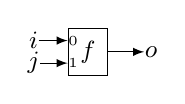
\begin{tikzpicture}[auto,>=latex,inner sep=0mm]
  \node[block, minimum height=.6cm, minimum width=.5cm] (function) {$f$};
  \node[below=1mm of function.north west,font=\tiny,anchor=north west] (0) {0};
  \node[above=1mm of function.south west,font=\tiny,anchor=south west] (1) {1};
  \node[left of=0, node distance=.5cm] (input0) {$i$};
  \node[left of=1, node distance=.5cm] (input1) {$j$};
  \node[right of=function, node distance=.8cm] (output) {$o$};
  \draw[->] (input0) -- (0);
  \draw[->] (input1) -- (1);
  \draw[->] (function) -- (output);
\end{tikzpicture}
\end{center}
\vspace{-1.2ex}
%
Most of the functions we deal with are commutative, so we can skip
inputs label, displaying the circuit above as:
%
\begin{center}
  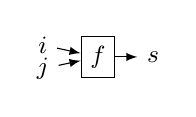
\begin{tikzpicture}[auto,>=latex, node distance=.7cm]
    \node[] (input0) {$i$};
    \node[below of=input0,node distance=.15cm] (dummy) {};
    \node[below of=dummy,node distance=.15cm] (input1) {$j$};
    \node[block, right of=dummy] (T) {$f$};
    \node[right of=T] (output) {$s$};
    \draw[->] (input0) -- (T);
    \draw[->] (input1) -- (T);
    \draw[->] (T) -- (output);
  \end{tikzpicture}
\end{center}
\vspace{-1.2ex}
%
Functions, and their circuits, can be composed, as in the following
example for the function $o = g(s) + (f(s) \times s)$:
%
\begin{center}
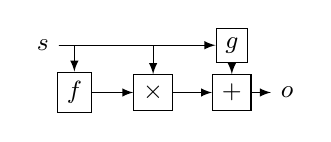
\begin{tikzpicture}[auto,>=latex]
  \node[] (input) {$s$};
  \node[] [right of=input, node distance=.4cm] (dummy) {};
  \node[block, below of=dummy, node distance=.6cm] (S1) {$f$};
  \node[block, right of=S1] (T1) {$\times$};
  \node[block, right of=T1] (T2) {$+$};
  \node[block, above of=T2, node distance=.6cm] (S2) {$g$};
  \node[right of=T2, node distance=.7cm] (output) {$o$};
  \draw[->] (input) -| (S1);
  \draw[->] (input) -| (T1);
  \draw[->] (S1) -- (T1);
  \draw[->] (T1) -- (T2);
  \draw[->] (input) -- (S2);
  \draw[->] (T2) -- (output);
  \draw[->] (S2) -- (T2);
\end{tikzpicture}
\end{center}
\vspace{-1ex}
%
We say that two circuits are \defined{equivalent} if they compute the
same function.  We use the symbol $\cong$ to indicate circuit
equivalence.  For example, we have the following circuit equivalence
(where $\circ$ is function composition):

\noindent
\begin{tabular}{m{3cm}m{.3cm}m{3cm}c}
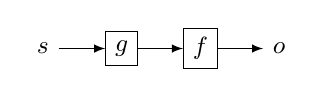
\begin{tikzpicture}[auto,>=latex]
  \node[] (input) {$s$};
  \node[block, right of=input] (g) {$g$};
  \node[block, right of=g] (f) {$f$};
  \node[right of=f] (output) {$o$};
  \draw[->] (input) -- (g);
  \draw[->] (g) -- (f);
  \draw[->] (f) -- (output);
\end{tikzpicture}
&
$\cong$
&
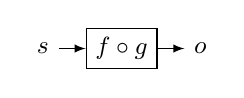
\begin{tikzpicture}[auto,>=latex]
    \node[] (input) {$s$};
    \node[block, right of=input, node distance=1cm] (fg) {$f \circ g$};
    \node[right of=fg, node distance=1cm] (output) {$o$};
    \draw[->] (input) -- (fg);
    \draw[->] (fg) -- (output);
\end{tikzpicture}
&
(*)
\end{tabular}
\vspace{-2ex}

\subsection{Streams}

The core notion of \dbsp is the \textbf{stream}.  Given a set $A$, a
\defined{stream} \emph{of values from $A$} is an infinite sequence of
values from $A$.  $\stream{A}$ denotes the set of all streams with
values from $A$.  We write $s[t]$ for the $t$-th element of the stream
$s$.  Think of $t$ as the ``time'' and of $s[t]\in A$ as the value of
the stream $s$ ``at time'' $t$.  We show streams as a sequence of
boxes, with time from \emph{right to left}: e.g., the stream $s[t] =
t$ is:
%
\begin{center}
\begin{tabular}{cc}
  \sv{0 1 2 3 4} \\
  $\xleftarrow[\hspace{1cm}\mathrm{time}\hspace{1cm}]{}$
\end{tabular}
\end{center}
\vspace{-1ex}
%
%\begin{definition}[stream operator]
A \defined{stream operator} is a function that computes on streams and
produces streams.
%\end{definition}
In general we use ``operator'' for streams, and ``function'' for
computations on ``scalar'' values.

We use arrows with a double head to depict streams.  The following
diagram shows a stream operator $T$ consuming two input streams $s_0$
and $s_1$, producing one output stream $s$:
%
\begin{center}
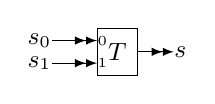
\begin{tikzpicture}[auto,>=latex,inner sep=0mm]
  \node[block, minimum height=.6cm, minimum width=.5cm] (function) {$T$};
  \node[below=1mm of function.north west,font=\tiny,anchor=north west] (0) {0};
  \node[above=1mm of function.south west,font=\tiny,anchor=south west] (1) {1};
  \node[left of=0, node distance=0.8cm] (input0) {$s_0$};
  \node[left of=1, node distance=0.8cm] (input1) {$s_1$};
  \node[right of=function, node distance=.8cm] (output) {$s$};
  \draw[->>] (input0) -- (0);
  \draw[->>] (input1) -- (1);
  \draw[->>] (function) -- (output);
\end{tikzpicture}
\vspace{-1ex}
\end{center}
%
We write $s = T(s_0, s_1)$.
%\begin{definition}(lifting)
Given a function $f: A \to B$, we define a stream operator $\lift{f}
:\stream{A} \to \stream{B}$ (read as ``$f$ lifted'') by applying
function $f$ to each input value independently:
\begin{center}
  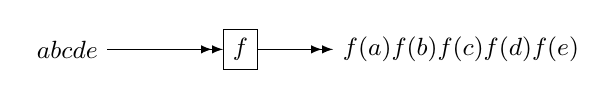
\begin{tikzpicture}[auto,>=latex]
    \node[] (input) {$\sv{a b c d e}$};
    \node[block, right of=input, node distance=2.2cm] (f) {$\lift{f}$};
    \node[right of=f, node distance=2.8cm] (output) {$\sv{f(a) f(b) f(c) f(d) f(e)}$};
    \draw[->>] (input) -- (f);
    \draw[->>] (f) -- (output);
  \end{tikzpicture}
\end{center}
\vspace{-1ex}
%\end{definition}

To simplify the notation, we write $a + b$ for streams $a, b$ instead
of $a (\lift{+}) b$; we also write $-a$ instead of $(\lift{-})a$.

\subsection{Databases as streams}

We generally think of streams as sequences of ``small'' values, such
as insertions or deletions in a database.  However, we also treat the
whole database as a \emph{stream of database snapshots}.  We model a
database as a stream $DB$.  Time is not wall-clock time, but counts
the transactions applied to the database.  Since transactions are
linearizable, they have a total order.  $DB[t]$ is the snapshot of the
database contents after $t$ transactions have been applied.  This
notation is apparent in the diagrams in \refsec{sec:intro-incremental}.

Database transactions also form a stream $\Delta DB$, this time a
stream of \emph{changes}, or \emph{deltas}, that are applied to the
database.  The values of this stream are defined by $(\Delta DB)[t] =
DB[t] - DB[t-1]$, where ``$-$'' stands for the difference between two
databases, a notion that we will soon make more precise.  The $\Delta
DB$ stream can be produced from the $DB$ stream by the \emph{stream
differentiation} operator $\D$; this operator produces as its output
the stream of changes from its input stream; we have thus $\D(DB) =
\Delta DB$.

Conversely, the database snapshot at time $t$ is the cumulative result
of applying all transactions up to $t$: $DB[t] = \Delta DB[0] + \Delta
DB[1] + \ldots + \Delta DB[t]$.  The stream operator $\I$ is defined
to produce each output by adding up all previous inputs.  We call $\I$
\emph{stream integration}, the inverse of differentiation.  The
following diagram shows the relationship between the streams $\Delta
DB$ and $DB$:
\begin{center}

\begin{tikzpicture}[auto,>=latex,minimum width=.5cm, node distance=1.2cm]
  \node[] (input) {$\Delta DB$};
  \node[block, right of=input] (I) {$\I$};
  \node[right of=I] (output) {$DB$};
  \node[block, right of=output] (D) {$\D$};
  \node[right of=D] (end) {$\Delta DB$};
  \draw[->>] (input) -- (I);
  \draw[->>] (I) -- (output);
  \draw[->>] (output) -- (D);
  \draw[->>] (D) -- (end);
\end{tikzpicture}
\end{center}

A view in this model is also a stream.  Suppose query $Q$ defining a
view $V$.  For each snapshot of the database stream we have a snapshot
of the view: $V[t] = Q(DB[t])$.  A view is thus just a lifted query:
$V = (\lift{Q})(DB)$.

Armed with these basic definitions, we can precisely define IVM.  What
does it mean to maintain a view incrementally?  A maintenance
algorithm needs to compute the \emph{changes} to the view given the
changes to the database. Given a query $Q$, a key contribution of this
paper is the definition of its \emph{incremental version} $\inc{Q}$,
using stream integration and differentiation, depicted graphically as:
\vspace{-2ex}
%
\begin{center}
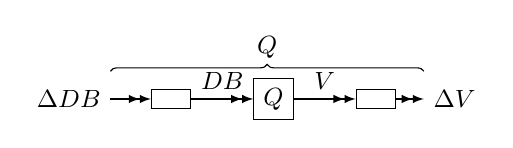
\begin{tikzpicture}[auto,>=latex,minimum width=.5cm]
  \node[] (input) {$\Delta DB$};
  \node[block, right of=input, node distance=1.3cm] (I) {$\I$};
  \node[block, right of=I, node distance=1.3cm] (Q) {$\lift{Q}$};
  \node[block, right of=Q, node distance=1.3cm] (D) {$\D$};
  \node[right of=D] (output) {$\Delta V$};
  \draw[->>] (input) -- (I);
  \draw[->>] (I) -- node (db) {$DB$} (Q);
  \draw[->>] (Q) -- node (B) {$V$} (D);
  \draw[->>] (D) -- (output);
  \draw[decorate, decoration = {brace, raise=10pt}] (input) -- (output)
  node[pos=.5, above=11pt]{$\inc{Q}$};
\end{tikzpicture}
\end{center}
\vspace{-1ex}
%
Mathematically: $\inc{Q} = \D \circ (\lift{Q}) \circ \I$.  The
incremental version of a query $Q$ is a \emph{streaming operator}
$\inc{Q}$ which computes directly on changes and produces changes.
The incremental version of a query is thus always well-defined.  The
above definition gives us one way to compute a query incrementally,
but applying it naively produces an inefficient execution, since it
reconstructs the database at each step.  It is in fact as bad as the
naive solution.  In \refsec{sec:incremental} we show how we can
optimize the implementation of $\inc{Q}$. The key property is that the
we can ``push'' the $\inc{.}$ operator ``down'' in a query plan:
$\inc{(Q_1 \circ Q_2)} = \inc{Q_1} \circ \inc{Q_2}$.

Armed with this general theory of incremental computation, in
\secref{sec:relational} we show how to model relational queries in
\dbsp.  This immediately gives us a general algorithm to compute the
incremental version of any relational query.  These results were
previously known, but they are cleanly modeled by \dbsp.
\secref{sec:recursion} shows how programs containing recursion can be
implemented and incrementalized in \dbsp.  For example, given an
implementation of transitive closure in the natural recursive way, our
algorithm produces a program that efficiently maintains the transitive
closure of a graph as nodes and edges are added and deleted.

\subsection{Contributions}

This work makes the following contributions:
\begin{enumerate}[nosep, leftmargin=0pt, itemindent=0.5cm, label=\textbf{(\arabic{*})}]
  \item We introduce \dbsp, a simple but expressive language for
    streaming computation. \dbsp gives an elegant formal foundation
    unifying the manipulation of streaming and incremental
    computations.
  \item An algorithm for incrementalizing any streaming computation
    expressed in \dbsp that handles arbitrary insertions and deletions
    from any of the data sources.
  \item An illustration of how \dbsp can model various classes of
    practical queries, such as relational algebra, nested relations,
    aggregations, and Datalog.
  \item The first general and machine-checked theory of IVM.  All the
    theoretical results in the original version of this
    paper~\cite{budiu-vldb23} have been checked~\cite{dbsp-theory}
    using the Lean proof assistant~\cite{moura-cade15}.
  \item A practical open-source implementation of this theory as a
    runtime and a SQL compiler.
\end{enumerate}


\section{Stream operators}\label{sec:streams}

%\subsection{Useful stream operators}\label{sec:abelian}

For the rest of this paper we require the set of values $A$ of a
stream $\stream{A}$ to form a commutative group, with operations $+$,
$-$, and a $0$ (zero) value.  The \emph{plus} defines what it means to
\emph{add} new data, while the \emph{minus} allows us to compute
differences (deltas).  We show later that this requirement is not a
problem for using \dbsp in the context of databases.

Stream operators are very powerful mathematically, but in \dbsp we
restrict ourselves to a very small subset.  All \dbsp computations are
\emph{causal}~\cite{causal}: the output at time $t$ is produced
immediately after all inputs up at time $t$ have been received; the
output at time $t$ cannot depend on inputs arriving after $t$.

The following circuit equivalence tells us that we can lift a circuit
by lifting each of its functions separately:

\noindent
\begin{tabular}{m{3cm}m{.3cm}m{3cm}c}
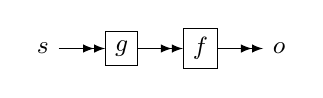
\begin{tikzpicture}[auto,>=latex]
  \node[] (input) {$s$};
  \node[block, right of=input] (g) {$\lift{g}$};
  \node[block, right of=g] (f) {$\lift{f}$};
  \node[right of=f] (output) {$o$};
  \draw[->>] (input) -- (g);
  \draw[->>] (g) -- (f);
  \draw[->>] (f) -- (output);
\end{tikzpicture}
&
$\cong$
&
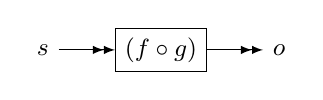
\begin{tikzpicture}[auto,>=latex]
    \node[] (input) {$s$};
    \node[block, right of=input, node distance=1.5cm] (fg) {$\lift{(f \circ g)}$};
    \node[right of=fg, node distance=1.5cm] (output) {$o$};
    \draw[->>] (input) -- (fg);
    \draw[->>] (fg) -- (output);
\end{tikzpicture}
&
(**)
\end{tabular}


%\subsubsection{Delays}\label{sec:delay}

%\begin{definition}[Delay]
The \defined{delay operator} $z^{-1}$ produces an output stream by
delaying its input by one step (and starting with a
zero)\footnote{This bizarre name comes from digital signal
processing.}:
%
\begin{center}
  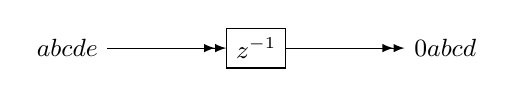
\begin{tikzpicture}[auto,>=latex,node distance=2.4cm]
    \node[] (input) {$\sv{a b c d e}$};
    \node[block, right of=input] (z) {$z^{-1}$};
    \node[right of=z] (output) {$\sv{0 a b c d}$};
    \draw[->>] (input) -- (z);
    \draw[->>] (z) -- (output);
  \end{tikzpicture}
\end{center}
\vspace{-1ex}
%\end{definition}
%
A very important property of the delay operator is that it produces
the first output \emph{before} having received the first input, and it
produces the second output before having received the second input,
etc.

%\begin{definition}[Time invariance]
%A stream operator $S: \stream{A} \to \stream{B}$ is \defined{time-invariant} (TI) if
%$S(\zm_A(s)) = \zm_B(S(s))$ for all $s \in \stream{A}$; in other words, if
%the following two circuits are equivalent:
%
%\begin{tabular}{m{3cm}m{.5cm}m{3cm}}
%\begin{tikzpicture}[auto,>=latex]
%  \node[] (input) {$s$};
%  \node[block, right of=input] (S) {$S$};
%  \node[block, right of=S] (z) {$\zm$};
%  \node[right of=z] (output) {$o$};
%  \draw[->] (input) -- (S);
%  \draw[->] (S) -- (z);
%  \draw[->] (z) -- (output);
%\end{tikzpicture}
%&
%$\cong$
%&
%\begin{tikzpicture}[auto,>=latex]
%  \node[] (input) {$s$};
%  \node[block, right of=input] (z) {$\zm$};
%  \node[block, right of=z] (S) {$S$};
%  \node[right of=S] (output) {$o$};
%  \draw[->] (input) -- (z);
%  \draw[->] (z) -- (S);
%  \draw[->] (S) -- (output);
%\end{tikzpicture}
%\end{tabular}
%
%\noindent
%This definition extends
%naturally to operators with multiple inputs.
%\end{definition}
%
%The composition of TI operators of any number of inputs
%is TI. The delay operator $\zm$ is TI.
%\dbsp only uses TI operators.
%
%%\begin{definition}
%%We say that a function between groups $f: A \to B$ has the \emph{zero-preservation
%%property} if $f(0_A) = 0_B$.  We write $\zpp{f}$.
%%\end{definition}
%%
%%A lifted operator $\lift{f}$ is TI iff $\zpp{f}$.
%
%\subsubsection{Causal and strict operators}\label{sec:causal}
%
%\begin{definition}[Causality]
%A stream operator $S:\stream{A}\to\stream{B}$
%is \defined{causal} when for all $s,s'\in\stream{A}$,
%and all times $t$ we have:
%$
%(\forall i \leq t . s[i]=s'[i]) ~~\Rightarrow~~ S(s)[t]=S(s')[t].
%$
%\end{definition}
%
%\noindent
%In other words, the output value at time $t$ can only depend on
%input values from times $t' \leq t$.
%Operators produced by lifting are causal, and $\zm$ is causal.
%All \dbsp operators are causal.  The composition
%of causal operators of any number of inputs is causal.
%
%\begin{definition}[Strictness]
%A stream operator, $F:\stream{A}\to\stream{B}$
%is \defined{strict}
%if  $\forall s,s'\in\stream{A}, \forall t \in \N$ we have:
%$(\forall i<t . ~s[i]=s'[i]) ~~\Rightarrow \\ F(s)[t]=F(s')[t].$
%\end{definition}
%
%In other words, the $t$-th output of $F(s)$ can depend only on ``past'' values
%of the input $s$, between $0$ and $t-1$.
%In particular, $F(s)[0] = 0_B$ is the same for all $s \in \stream{A}$.
%Strict operators are causal. Lifted operators in general are \emph{not} strict.
%$\zm$ is strict.  %In \dbsp $\zm$ is the only primitive strict operator.
%
%\begin{proposition}
%\label{prop-unique-fix}
%For a strict $F: \stream{A} \to \stream{A}$ the equation ~$\alpha=F(\alpha)$~ has a unique
%solution $\alpha \in \stream{A}$, denoted by $\fix{\alpha}{F(\alpha)}$.
%\end{proposition}
%
%Thus every strict operator from a set to itself has a unique fixed
%point.  The simple proof relies on strong induction, showing that the
%solution $\alpha[t]$ depends only on the values of $\alpha$ prior to
%$t$.
%
%Consider a circuit with a strict feedback edge:
%\begin{center}
%\begin{tikzpicture}[>=latex]
%    \node[] (input) {$s$};
%    \node[block, right of=input] (f) {$T$};
%    \node[right of=f] (output) {$\alpha$};
%    \node[block, below of=f, node distance=.5cm] (z) {$F$};
%    \draw[->] (input) -- (f);
%    \draw[->] (f) -- node (mid) {} (output);
%    \draw[->] (mid.center) |-  (z);
%    \draw[->] (z.west) -- ++(-.3,0) |- ([yshift=1mm]f.south west);
%\end{tikzpicture}
%\end{center}
%
%This circuit is a well-defined function on streams:
%
%%\begin{lemma}
%%\label{lemma-causal-strict}
%%If $F: \stream{B} \to \stream{B}$ is strict and $T: \stream{A} \times \stream{B} \to \stream{B}$ is causal, then for fixed $s$ the operator
%%$\lambda\alpha.T(s,F(\alpha)): \stream{A} \to \stream{B}$ is strict.
%%\end{lemma}
%
%\begin{lemma}\label{feedback-semantics}
%\label{cor-loop}
%If $F: \stream{B} \to \stream{B}$ is strict and $T: \stream{A} \times \stream{B} \to \stream{B}$ is causal,
%the operator $Q(s)=\fix{\alpha}{T(s,F(\alpha))}$ is well-defined and causal.
%If, moreover, $F$ and $T$ are TI then so is $Q$.
%\end{lemma}
%
%All \dbsp computations are built using just lifted functions and
%delays.  We add two more operators in \secref{sec:nested}.
%
%\subsection{Integration and differentiation}\label{sec:abelianstreams}

%Remember that we require the elements of a stream to come from an abelian group $A$.
%Streams themselves form an abelian group:
%
%\begin{proposition}
%The structure $(\stream{A},+,0,-)$, obtained by lifting the $+$ and unary $-$ operations of $A$,
%is an abelian group.  0 is the stream with all values $0_A$.
%\end{proposition}
%
%\noindent
%Stream addition and negation are causal, TI operators.

%Given a linear function $f: A \to B$, the stream operator $\lift{f}$
%is linear and TI (LTI).  $\zm$ is also LTI.
%
%\begin{definition}(bilinear)
%A function of two arguments $f: A \times B \to C$ with $A, B, C$ groups, is \emph{bilinear}
%if it is linear separately in each argument (i.e., it distributes over addition):
%$\forall a, b, c, d . f(a+b, c) = f(a, c) + f(b, c)$, and $f(a, c+d) = f(a, c) + f(c, d).$
%\end{definition}
%
%This definition extends to stream operators.
%The lifting of a bilinear function $f$ is
%a bilinear stream operator $\lift{f}$.  An example
%is lifted multiplication:
%$f: \stream{\N} \times \stream{\N} \to \stream{\N}, f(a, b)[t] = a[t]\cdot b[t]$.

%The composition of (bi)linear operators with linear operators
%is (bi)linear (since homomorphisms compose).

%The ``feedback loop'' of a linear operator is linear:
%
%\begin{proposition}
%\label{prop-rec-linear}
%Let $S$ be a unary, causal, LTI operator. The
%operator $Q(s)=\fix{\alpha}{S(s+\zm(\alpha))}$ is well-defined and LTI:
%
%\begin{center}
%\begin{tikzpicture}[>=latex]
%    \node[] (input) {$s$};
%    \node[block, shape=circle, right of=input, inner sep=0pt, node distance=.6cm] (plus) {$+$};
%    \node[block, right of=plus, node distance=.6cm] (Q) {$S$};
%    \node[right of=Q, node distance=1.2cm] (output) {$\alpha$};
%    \node[block, below of=Q, node distance=.6cm] (z) {$\zm$};
%    \draw[->] (input) -- (plus);
%    \draw[->] (plus) -- (Q);
%    \draw[->] (Q) -- node (mid) {} (output);
%    \draw[->] (mid.center) |-  (z);
%    \draw[->] (z) -| (plus);
%\end{tikzpicture}
%\end{center}
%\end{proposition}

%\begin{definition}[Differentiation]
We define the \defined{differentiation operator} as a composition of
several other operators: $\D(s) \defn s - \zm(s)$, shown as:
%
\vspace{-2ex}
\begin{center}
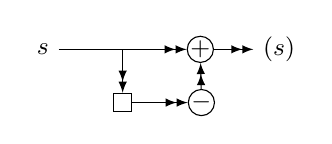
\begin{tikzpicture}[auto,>=latex,node distance=1cm]
    \node[] (input) {$s$};
    \node[block, shape=circle, right of=input, inner sep=0pt,node distance=2cm] (plus) {$+$};
    \node[right of=plus] (output) {$\D(s)$};
    \draw[->>] (input) -- node (i) {} (plus);
    \node[block, below of=i, node distance=.8cm] (z) {$\zm$};
    \node[block, shape=circle, right of=z, inner sep=0pt] (minus) {$-$};
    \draw[->>] (plus) -- (output);
    \draw[->>] (i) -- (z);
    \draw[->>] (z) -- (minus);
    \draw[->>] (minus) -- (plus);
\end{tikzpicture}
\end{center}
%\end{definition}
%We generally omit the type, and write just $\D$.
%The value of $\D(s)[t] = s[t] - s[t-1]$ if $t > 0$.
%
If $s$ is a stream, then $\D(s)$ is the \emph{stream of changes} of
$s$; a value in the output is the difference between two consecutive
values in the input.  As an example:
{
\noindent \small
\begin{align*}
  &\D(\sv{0 1 2 1 0}) &= \\
  &\sv{0 1 2 1 0} - \zm(\sv{0 1 2 1 0}) &=\\
  &\sv{0 1 2 1 0} - \sv{0 0 1 2 1} &=\\
%  &\sv{0-0 1-0 2-1 1-2 0-1} =\\
  &\sv{0 1 1 -1 -1}
\end{align*}
}

%\begin{proposition}
%\label{prop-diff-properties}
%$\D$ is causal and LTI.
%\end{proposition}

%The integration operator ``reconstitutes'' a stream from its changes:

%\begin{definition}[Integration]
The \defined{integration operator}
is given by the following circuit:
\vspace{-2ex}
\begin{center}
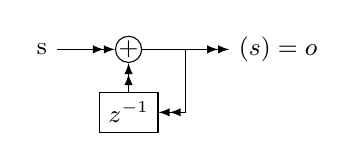
\begin{tikzpicture}[auto,>=latex, node distance=1.1cm]
    \node[] (input) {s};
    \node[block, shape=circle, right of=input, inner sep=0pt] (plus) {$+$};
    \node[right of=plus, node distance=1.9cm] (output) {$\I(s) = o$};
    \node[block, below of=plus, node distance=.8cm] (z) {$z^{-1}$};
    \draw[->>] (input) -- (plus);
    \draw[->>] (plus) -- node (o) {} (output);
    \draw[->>] (o) |- (z);
    \draw[->>] (z) -- (plus);
\end{tikzpicture}
\end{center}
\vspace{-1ex}
%\end{definition}
%
While this definition may seem strange, because the output stream is
used to compute itself, the use of the delay in the ``feedback'' loop
ensures that only \emph{previous} values of the output are used in
computing the current one.  Using the notation $o = \I(s)$ to make
formulas more readable, we can see the contents of stream $o$ is
produced step by step:
\begin{align*}
  o[0] &= s[0] + (\zm(o))[0] = s[0] + 0 = s[0] \\
  o[1] &= s[1] + (\zm(o))[1] = s[1] + o[0] = s[1] + s[0] \\
  o[2] &= s[2] + (\zm(o))[2] = s[2] + o[1] = s[2] + (s[1] + s[0])
\end{align*}

%\noindent
%We also generally omit the type, and write just $\I$.
%This is the construction from Proposition~\ref{prop-rec-linear}
%using the identity function for $S$.
%
%\begin{proposition}
%$\I(s)$ is the discrete (indefinite) integral applied to the stream $s$:
%\end{proposition}
In general, $\I(s)[t] = o[t] = \sum_{i \leq t} s[i]$.
Examples:
\begin{align*}
  \I(\sv{0 1 2 3 4 5}) &= \sv{0 1 3 6 10} \\
  \I(\sv{0 1 1 -1 -1}) &= \sv{0 1 2 1 0}.
\end{align*}

%\begin{proposition}
%\label{prop-integ-properties}
%$\I$ is causal and LTI.
%\end{proposition}
%
%\begin{theorem}[Inversion]
%\label{inverses}
%Integration and differentiation are inverses of each other:
%$\forall s . \I(\D(s)) = \D(\I(s)) = s$.
%\end{theorem}

Integration and differentiation are inverses of each other: while $\D$
computes the changes of a stream, $\I$ reconstitutes the original
stream given the stream of changes.  $\I$ and $\D$ ``cancel out'' when
applied in sequence:

\noindent
\begin{tabular}{m{2.5cm}m{.3cm}m{1cm}m{.3cm}m{2.5cm}}
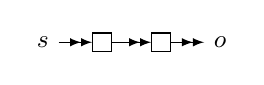
\begin{tikzpicture}[auto,>=latex, node distance=.75cm]
    \node[] (input) {$s$};
    \node[block, right of=input] (I) {$\I$};
    \node[block, right of=I] (D) {$\D$};
    \node[right of=D] (output) {$o$};
    \draw[->>] (input) -- (I);
    \draw[->>] (I) -- (D);
    \draw[->>] (D) -- (output);
\end{tikzpicture}
     &
     $\cong$
     &
     \hspace{-2ex}
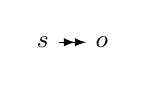
\begin{tikzpicture}[auto,>=latex, node distance=.75cm]
    \node[] (input) {$s$};
    \node[right of=input] (output) {$o$};
    \draw[->>] (input) -- (output);
\end{tikzpicture}
     &
     $\cong$
     &
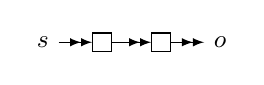
\begin{tikzpicture}[auto,>=latex, node distance=.75cm]
    \node[] (input) {$s$};
    \node[block, right of=input] (D) {$\D$};
    \node[block, right of=D] (I) {$\I$};
    \node[right of=I] (output) {$o$};
    \draw[->>] (input) -- (D);
    \draw[->>] (D) -- (I);
    \draw[->>] (I) -- (output);
\end{tikzpicture}
\end{tabular}

\section{Incremental view maintenance}\label{sec:incremental}

The results in this section are not specific to databases, they hold
for any stream computations, but we hint about their applicability for
databases.

%Here we define IVM and analyze its properties.

%\begin{definition}
Given a stream operator $S: \stream{A} \to \stream{B}$ we define the
\defined{incremental version} of $S$ as:
%\begin{equation}\label{def:inc}
%\inc{Q} \defn \D \circ Q \circ \I.
%\end{equation}
%$\inc{Q}$ has the same ``type'' as $Q$: $\inc{Q}: \stream{A} \to \stream{B}$.

%The following diagram illustrates the intuition behind this
%definition:
\vspace{-2ex}
\begin{center}
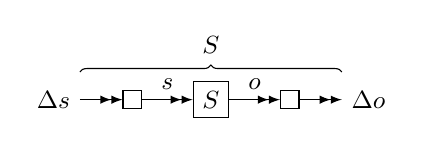
\begin{tikzpicture}[auto,>=latex]
    \node[] (input) {$\Delta s$};
    \node[block, right of=input] (I) {$\I$};
    \node[block, right of=I] (Q) {$S$};
    \node[block, right of=Q] (D) {$\D$};
    \node[right of=D] (output) {$\Delta o$};
    \draw[->>] (input) -- (I);
    \draw[->>] (I) -- node (s) {$s$} (Q);
    \draw[->>] (Q) -- node (o) {$o$} (D);
    \draw[->>] (D) -- (output);
    \draw[decorate, decoration = {brace, raise=10pt}] (input) -- (output)
    node[pos=.5, above=13pt]{$\inc{S}$};
\end{tikzpicture}
\end{center}
\vspace{-1ex}
%\end{definition}

If $S$ computes on a stream $s$, then $\inc{S}$ computes on a stream
of changes to $s$.  If $S$ produces a stream $o$, then $\inc{S}$
produces the stream of changes to $o$.  Note that this definition does
not require $S$ to be a lifted function.

For an operator with multiple inputs and outputs we define the
incremental version by applying $\I$ to each input, and $\D$ to each
output, e.g.: $\inc{T}(a, b) \defn \D (T(\I(a), \I(b)))$.

%Notice that our definition of incremental computation is meaningful only for \emph{streaming}
%computations; this is in contrast to classic definitions, e.g.~\cite{gupta-idb95} which
%consider only one change.  Generalizing the definition to operate on streams gives us
%additional power, especially when operating with recursive queries.
%
%The following proposition is one of our central results:
$\inc{S}$ has many nice properties:

%\begin{proposition}(Properties of the incremental version):
%\label{prop-inc-properties}
%\begin{description}
%\item[inversion:] $Q\mapsto\inc{Q}$ is bijective; its inverse is $Q\mapsto \I\circ Q\circ\D$.
%\item[invariance:] $\inc{+} = +, \inc{(\zm)} = \zm, \inc{-} = -, \inc{\I}=\I, \inc{\D}=\D$
%\item[push/pull:] \label{prop-part-commutation}
%    $Q \circ \I = \I \circ \inc{Q}$; $\D\circ Q = \inc{Q}\circ\D$
%\item[chain:] $\inc{(Q_1\circ Q_2)} = \inc{Q_1}\circ\inc{Q_2}$ (Generalizes to multiple inputs.)
%\item[add:] $\inc{(Q_1 + Q_2)} = \inc{Q_1} + \inc{Q_2}$
%\item[cycle:] $\inc{(\lambda s. \fix{\alpha}{T(s,\zm(\alpha)}))} = \lambda s. \fix{\alpha}{\inc{T}(s,\zm(\alpha)})$
%\end{description}
%\end{proposition}
%
The \defined{chain rule} states that $\inc{(Q_1 \circ Q_2)} =
\inc{Q_1} \circ \inc{Q_2}$, i.e., these circuits are equivalent:

\noindent
\begin{tabular}{cr}
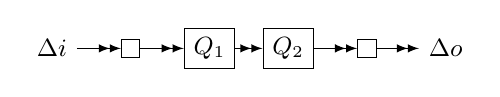
\begin{tikzpicture}[auto,>=latex]
  \node[] (input) {$\Delta i$};
  \node[block, right of=input] (I) {$\I$};
  \node[block, right of=I] (Q1) {$Q_1$};
  \node[block, right of=Q1] (Q2) {$Q_2$};
  \node[block, right of=Q2] (D) {$\D$};
  \node[right of=D] (output)  {$\Delta o$};
  \draw[->>] (input) -- (I);
  \draw[->>] (I) -- (Q1);
  \draw[->>] (Q1) -- (Q2);
  \draw[->>] (Q2) -- (D);
  \draw[->>] (D) -- (output);
\end{tikzpicture} &
$\cong$ \\
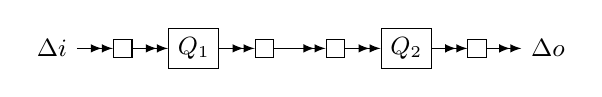
\begin{tikzpicture}[>=latex, node distance=.9cm]
  \node[] (input) {$\Delta i$};
  \node[block, right of=input] (I1) {$\I$};
  \node[block, right of=I1] (Q1) {$Q_1$};
  \node[block, right of=Q1] (D1) {$\D$};
  \node[block, right of=D1] (I2) {$\I$};
  \node[block, right of=I2] (Q2) {$Q_2$};
  \node[block, right of=Q2] (D2) {$\D$};
  \node[right of=D2] (output)  {$\Delta o$};
  \draw[->>] (input) -- (I1);
  \draw[->>] (I1) -- (Q1);
  \draw[->>] (Q1) -- (D1);
  \draw[->>] (D1) -- (I2);
  \draw[->>] (I2) -- (Q2);
  \draw[->>] (Q2) -- (D2);
  \draw[->>] (D2) -- (output);
\end{tikzpicture} &
$\cong$ \\
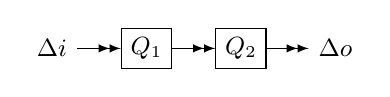
\begin{tikzpicture}[>=latex, node distance=1.2cm]
  \node[] (input) {$\Delta i$};
  \node[block, right of=input] (Q1) {$\inc{Q_1}$};
  \node[block, right of=Q1] (Q2) {$\inc{Q_2}$};
  \node[right of=Q2] (output)  {$\Delta o$};
  \draw[->>] (input) -- (Q1);
  \draw[->>] (Q1) -- (Q2);
  \draw[->>] (Q2) -- (output);
\end{tikzpicture}
\end{tabular}

\noindent In the database world, we can read this as: \textbf{to
  incrementalize a composite query you can incrementalize each
  sub-query independently}.  This gives us a simple deterministic
recipe reducing the incremental version of an arbitrary query to the
incremental version of its primitive operators.

The \defined{cycle rule} states that these circuits are equivalent:

\noindent
\begin{tabular}{m{4.4cm}m{.2cm}m{3cm}}
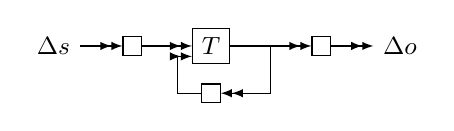
\begin{tikzpicture}[>=latex]
    \node[] (input) {$\Delta s$};
    \node[block, right of=input] (I) {$\I$};
    \node[block, right of=I] (f) {$T$};
    \node[block, right of=f, node distance=1.4cm] (D) {$\D$};
    \node[right of=D] (output) {$\Delta o$};
    \node[block, below of=f, node distance=.6cm] (z) {$\zm$};
    \draw[->>] (input) -- (I);
    \draw[->>] (I) -- (f);
    \draw[->>] (f) -- node (mid) {} (D);
    \draw[->>] (mid.center) |-  (z);
    \draw[->>] (z.west) -- ++(-.3,0) |- ([yshift=1mm]f.south west);
    \draw[->>] (D) -- (output);
\end{tikzpicture} & $\cong$ &
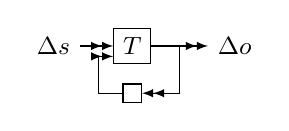
\begin{tikzpicture}[>=latex]
    \node[] (input) {$\Delta s$};
    \node[block, right of=input] (f) {$\inc{T}$};
    \node[right of=f, node distance=1.3cm] (output) {$\Delta o$};
    \node[block, below of=f, node distance=.6cm] (z) {$\zm$};
    \draw[->>] (input) -- (f);
    \draw[->>] (f) -- node (mid) {} (output);
    \draw[->>] (mid.center) |-  (z);
    \draw[->>] (z.west) -- ++(-.3,0) |- ([yshift=1mm]f.south west);
\end{tikzpicture}
\end{tabular}

\noindent
(We have omitted the labels on the inputs of $T$.) In other words, the
incremental version of a feedback loop around a query is just the
feedback loop with the incremental query for its body.  This result
will be useful for recursive queries.

%To execute incremental queries efficiently, we want to compute directly
%on streams of changes, without integrating them. The invariance property above shows
%that stream operators $+$, $-$, and $\zm$ are identical to their incremental versions.
%The following theorems generalize this to linear and bi-linear operators:

We call an operator $S$ \defined{linear} if it has the property that
$S(a+b) = S(a) + S(b)$ (where $+$ is the addition of streams).
%
%\begin{theorem}[Linear]\label{linear}
For a linear operator $S$ we have $\inc{S}=S$.
%\end{theorem}
%
This is very useful because many primitive database operations can be
implemented as linear operators: selection, projection, filtering,
grouping, parts of aggregation are all linear.  Moreover, the
following operators are linear: $-$, $z^{-1}$, $\I$, $\D$, $\lift{f}$
if $f$ is a linear function.

We call an operator $T$ with two inputs \defined{bilinear} if it
distributes over stream addition: $T(a+b, c) = T(a, c) + T(b, c)$, and
$T(a, c+d) = T(a, c) + T(a, d)$.  (Similar to multiplication's
distributivity over addition.)  In databases intersection, joins, and
Cartesian products are bilinear.

%\begin{theorem}[Bilinear]\label{bilinear}
Using infix notation, for a bilinear operator $\times$ we have:
\begin{eqnarray*}
\inc{(\Delta a \times \Delta b)} = \\
(\Delta a \times \Delta b ~+~ \zm(\I(\Delta a)) \times
\Delta b ~+~ \Delta a \times \zm(\I(\Delta b)) = \\
\Delta a \times \Delta b + \zm(a) \times \Delta b + \Delta a \times \zm(b)
\end{eqnarray*}

If we ignore the delay operators in this equation we recover the
well-known formula for join delta queries, e.g.,\cite{koch-pods10}.

%In pictures: \\
\noindent
\begin{tabular}{m{3.3cm}m{0cm}m{4cm}%m{0cm}m{2.8cm}
  }
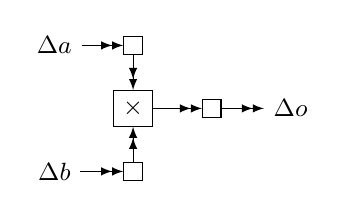
\begin{tikzpicture}[auto,>=latex]
    \node[] (a) {$\Delta a$};
    \node[block, right of=a] (ai) {$\I$};
    \node[below of=a, node distance=.8cm] (midway) {};
    \node[below of=midway, node distance=.8cm] (b) {$\Delta b$};
    \node[block, right of=b] (bi) {$\I$};
    \node[block, right of=midway, node distance=1cm] (q) {$\times$};
    \node[block, right of=q] (D) {$\D$};
    \node[right of=D] (output) {$\Delta o$};
    \draw[->>] (a) -- (ai);
    \draw[->>] (b) -- (bi);
    \draw[->>] (ai) -- (q);
    \draw[->>] (bi) -- (q);
    \draw[->>] (q) -- (D);
    \draw[->>] (D) -- (output);
\end{tikzpicture} &
$\cong$ &
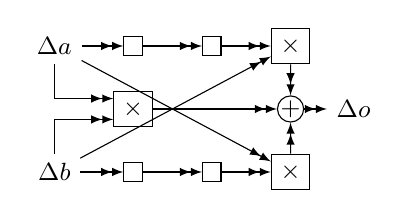
\begin{tikzpicture}[auto,>=latex]
  \node[] (input1) {$\Delta a$};
  \node[below of=input1, node distance=1.6cm] (input2) {$\Delta b$};
  \node[block, right of=input1, node distance=1cm] (I1) {$\I$};
  \node[block, below of=I1,node distance=.8cm] (ab) {$\times$};
  \node[block, right of=input2, node distance=1cm] (I2) {$\I$};
  \draw[->>] (input1) -- (I1);
  \draw[->>] (input2) -- (I2);
  \draw[->>] (input1) |- ([yshift=-1mm]ab.north west);
  \draw[->>] (input2) |- ([yshift=1mm]ab.south west);
  \node[block, right of=I1] (ZI1) {$\zm$};
  \node[block, right of=I2] (ZI2) {$\zm$};
  \draw[->>] (I1) -- (ZI1);
  \draw[->>] (I2) -- (ZI2);
  \node[block, right of=ZI1] (DI1) {$\times$};
  \node[block, right of=ZI2] (DI2) {$\times$};
  \draw[->>] (ZI1) -- (DI1);
  \draw[->>] (ZI2) -- (DI2);
  \node[block, circle, right of=ab, inner sep=0cm, node distance=2cm] (sum) {$+$};
  \draw[->>] (ab) -- (sum);
  \draw[->>] (DI1) -- (sum);
  \draw[->>] (DI2) -- (sum);
  \node[right of=sum, node distance=.8cm] (output) {$\Delta o$};
  \draw[->>] (sum) -- (output);
  \draw[->>] (input1) -- (DI2);
  \draw[->>] (input2) -- (DI1);
\end{tikzpicture}
%&
%$\cong$ &
%\begin{tikzpicture}[auto,>=latex,node distance=.7cm]
%  \node[] (input1) {$a$};
%  \node[below of=input1, node distance=1cm] (input2) {$b$};
%  \node[block, right of=input1, node distance=.5cm] (I1) {$\I$};
%  \node[block, right of=input2, node distance=.5cm] (I2) {$\I$};
%  \draw[->>] (input1) -- (I1);
%  \draw[->>] (input2) -- (I2);
%  \node[block, right of=I2] (ZI2) {$\zm$};
%  \draw[->>] (I2) -- (ZI2);
%  \node[block, right of=I1] (DI1) {$\times$};
%  \node[block, right of=ZI2] (DI2) {$\times$};
%  \draw[->>] (I1) -- (DI1);
%  \draw[->>] (ZI2) -- (DI2);
%  \node[block, circle, above of=DI2, inner sep=0cm, node distance=.5cm] (sum) {$+$};
%  \draw[->>] (DI1) -- (sum);
%  \draw[->>] (DI2) -- (sum);
%  \node[right of=sum, node distance=.5cm] (output) {$o$};
%  \draw[->>] (sum) -- (output);
%  \draw[->>] (input1) -- (DI2);
%  \draw[->>] (input2) -- (DI1);
%\end{tikzpicture}
\end{tabular}
%\end{theorem}

What is the intuition behind this diagram?  Let us consider the case
of Cartesian product $a \times b$.  The incremental product has inputs
$\Delta a = \D(a)$ and $\Delta b = \D(b)$.  What happens when we add a
row $x$ to relation $a$ (i.e., $\Delta a = x$)?  The new row $x$ will
appear in the output change combined with every row in the
\emph{previous version} of the \emph{full} relation $b$.  The operator
$\I(\Delta b)$ in fact computes relation $b$ from the stream $\Delta
b$ of changes, and $\zm$ applied to this value gives us its previous
version.  So the bottom $\times$ operator computes $x \times \zm(b) =
\Delta a \times \zm(\I(\Delta b))$, the change produced by the new row
$x$.  The top $\times$ operator performs the symmetric operation for
the changes of the $b$ relation.  The middle $\times$ operator
produces the results of changes to both inputs.

%Rewriting this statement using $\Delta a$ for the stream of changes to
%$a$ we get the familiar formula for incremental equi-joins:
%$\Delta(a\times b) =\Delta a \times \Delta b + a\times(\Delta b) +
%(\Delta a)\times b$; equi-joins are indeed bilinear.
%

\section{IVM for the Relational Algebra}\label{sec:relational}

Results in \secref{sec:streams} and~\secref{sec:incremental}
apply to streams of arbitrary group values.  In this
section we apply these results to
IVM for relational databases.  As explained in the introduction, our goal is to
efficiently compute the incremental version of any relational query $Q$
that defines a database view.

However, we face a technical problem: the $\I$ and $\D$ operators were
defined on abelian groups, and relational databases in general are
not abelian groups, since they operate on sets.  Fortunately,
there is a well-known tool in the database literature
which converts set operations into group operations by using \zrs
(also called z-relations~\cite{green-tcs11}) to represent sets.

We start by defining the \zrs group, and then we review how
relational queries are converted into \dbsp circuits  over \zrs.
This translation is efficiently incrementalizable because
many basic relational queries can be expressed using LTI \zr operators~\refsec{sec:relational-operators}.

\subsection{\zrs as an abelian group}

\zrs generalize database tables: think of a \zr as a table where each
row has an associated weight, possibly negative.

Given a set $A$, we define \defined{\zrs} over $A$ as functions with
\emph{finite support} from $A$ to $\Z$.  These are functions $f: A
\rightarrow \Z$ where $f(x) \not= 0$ for at most a finite number of
values $x \in A$.  We also write $\Z[A]$ for the type of \zrs with
elements from $A$.  Values in $\Z[A]$ can be thought of as key-value
maps with keys in $A$ and values in $\Z$, justifying the array
indexing notation.  If $m \in \Z[A]$ we write $m[a]$ instead of
$m(a)$, again using an indexing notation.

A particular \zr $m \in \Z[A]$ can be denoted by enumerating its
elements that have non-zero weights and their corresponding weights:
$m = \{ x_1 \mapsto w_1, \dots, x_n \mapsto w_n \}$.
We call $w_i \in \Z$ the \defined{weight}
of $x_i \in A$.  Weights can be negative.
We write that $x \in m$ iff $m[x] \not= 0$.
We also write $w \cdot x$ for $\{ x \mapsto w \}$.

\ifzsetexamples
Consider a concrete \zr $R \in \Z[\texttt{string}]$,
defined by $R = \{ \texttt{joe} \mapsto 1, \texttt{anne} \mapsto -1 \}$.
$R$ has two elements in its domain,
\texttt{joe} with weight 1 (so $R[\texttt{joe}] = 1$),
and \texttt{anne} with weight $-1$.
We say \texttt{joe} $\in R$ and \texttt{anne} $\in R$.
\fi

Since $\Z$ is an abelian ring, $\Z[A]$ is also an abelian ring (and thus a group).  This group
$(\Z[A], +_{\Z[A]}, 0_{\Z[A]}, -_{\Z{A}})$ has addition and subtraction defined pointwise:
$(f +_{\Z[A]} g)(x) = f(x) + g(x) . \forall x \in A.$
The $0$ element of $\Z[A]$ is the function $0_{\Z[A]}$ defined by $0_{\Z[A]}(x) = 0 .
\forall x \in A$.  For example, $R + R =  \{ \texttt{joe} \mapsto 2, \texttt{anne} \mapsto -2 \}$.
Since \zrs form a group, all results from \secref{sec:streams} apply to streams over \zrs.

\zrs generalize sets and bags.  A set with elements from $A$
can be represented as a \zr by associating a weight of 1 with each element.
Bags are \zrs where all weights are positive.  Crucially, \zrs
can also represent arbitrary \emph{changes} to sets and bags.
Negative weights in a change represent elements that are being ``removed''.

\begin{definition}
We say that a \zr represents a \defined{set} if the weight of every
element is one.  We define a function to check this property
$\isset : \Z[A] \rightarrow \B$\index{isset}
given by:
$$\isset(m) \defn \left\{
\begin{array}{ll}
  \mbox{true} & \mbox{ if } m[x] = 1, \forall x \in m \\
  \mbox{false} & \mbox{ otherwise}
\end{array}
\right.
$$
\end{definition}

\ifzsetexamples
For our example $\isset(R) = \mbox{false}$, since $R[\texttt{anne}] = -1$.
\fi

\begin{definition}
We say that a \zr is \defined{positive} (or a \defined{bag}) if the weight of every element is
positive.  We define a function to check this property
$\ispositive : \Z[A] \rightarrow \B$\index{ispositive}.
given by
$$\ispositive(m) \defn \left\{
\begin{array}{ll}
  \mbox{true} & \mbox{ if } m[x] \geq 0, \forall x \in A \\
  \mbox{false} & \mbox{ otherwise}
\end{array}
\right.$$
\end{definition}
We have $\forall m \in \Z[A] . \isset(m) \Rightarrow \ispositive(m)$.
\ifzsetexamples
$\ispositive(R) = \mbox{false}$, since $R[\texttt{anne}] = -1$.
\fi

We write $m \geq 0$ when $m$ is positive.  For positive $m, n \in
\Z[A]$ we write $m \geq n$ for iff $m - n \geq 0$.  $\geq$ is a
partial order.

We call a function $f : \Z[A] \rightarrow \Z[B]$ \defined{positive} if it maps
positive values to positive values:
$\forall x \in \Z[A], x \geq 0_{\Z[A]} \Rightarrow f(x) \geq 0_{\Z[B]}$.
We use the same notation for functions: $\ispositive(f)$.

\begin{definition}[distinct]
The function $\distinct: \Z[A] \rightarrow \Z[A]$\index{distinct}
``converts'' a \zr into a set:
$$\distinct(m)[x] \defn \left\{
\begin{array}{ll}
  1 & \mbox{ if } m[x] > 0 \\
  0 & \mbox{ otherwise}
\end{array}
\right.
$$
\end{definition}

Notice that $\distinct$ ``removes'' duplicates from multisets, and it also eliminates
elements with negative weights.
\ifzsetexamples
$\distinct(R) = \{ \texttt{joe} \mapsto 1 \}$.
\fi
While very simple, this definition of $\distinct$ has been carefully
chosen to enable us to implement the relational (set) operators
using \zrs operators.
%Circuits derived from relational queries only compute on positive \zrs.

%\begin{definition}(mononotonicity)
%A stream $s \in \stream{\Z[A]}$ is \defined{positive} if every value of the stream is positive:
%$s[t] \geq 0 . \forall t \in \N$.
%A stream $s \in \stream{\Z[A]}$ is \defined{monotone} if $s[t] \geq s[t-1], \forall t \in \N$.
%\end{definition}
%
%If $s \in \stream{\Z[A]}$ is positive, then $\I(s)$ is monotone.
%If $s \in \stream{\Z[A]}$ is monotone, $\D(s)$ is positive.
%
\paragraph{Generalizing circuit diagrams}

From now on we will use circuits to compute both on scalars (\zrs in our case) and streams of \zrs.
We use the same graphical representation for functions on streams or scalars:
boxes with input and output arrows.  For scalar functions the ``values''
of the arrows are scalars instead of streams; otherwise
the interpretation of boxes as function application is unchanged.  We will
thus use circuits to depict relational query plans.

\subsection{Implementing relational operators}\label{sec:relational-operators}

The fact that relational algebra can be implemented by computations
on \zrs has been shown before, e.g.~\cite{green-pods07}.  The translation
of the relational operators to \dbsp is shown in Table~\ref{tab:relational}.
The first row of the table shows that a composite query is translated
recursively.  This gives us a recipe for
translating an arbitrary relational query plan into a \dbsp circuit.

\newlength{\commentsize}
\setlength{\commentsize}{5cm}
\begin{table*}[h]
\small
\caption{Implementation of SQL relational set operators in \dbsp.
Each query assumes that inputs \code{I}, \code{I1}, \code{I2}, are sets and it
produces output sets.\label{tab:relational}}
\begin{tabular}{|m{1.2cm}m{4.2cm}m{5cm}m{\commentsize}|} \hline
Operation & SQL example & \dbsp circuit & Details \\ \hline
Composition &
 \begin{lstlisting}[language=SQL]
SELECT DISTINCT ... FROM
(SELECT ... FROM ...)
\end{lstlisting}
 &
 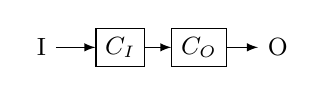
\begin{tikzpicture}[auto,>=latex]
  \node[] (I) {\code{I}};
  \node[block, right of=I] (CI) {$C_I$};
  \draw[->] (I) -- (CI);
  \node[block, right of=CI] (CO) {$C_O$};
  \node[right of=CO] (O) {\code{O}};
  \draw[->] (CI) -- (CO);
  \draw[->] (CO) -- (O);
\end{tikzpicture}
 &
 \parbox[b][][t]{\commentsize}{
  $C_I$ circuit for inner query, \\
  $C_O$ circuit for outer query.}
\\ \hline
Union &
\begin{lstlisting}[language=SQL]
(SELECT * FROM I1)
UNION
(SELECT * FROM I2)
\end{lstlisting}
&
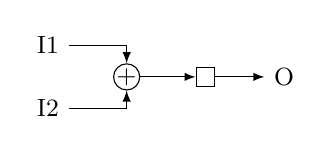
\begin{tikzpicture}[auto,>=latex]
  \node[] (input1) {\code{I1}};
  \node[below of=input1, node distance=.4cm] (midway) {};
  \node[below of=midway, node distance=.4cm] (input2) {\code{I2}};
  \node[block, shape=circle, right of=midway, inner sep=0in] (plus) {$+$};
  \node[block, right of=plus] (distinct) {$\distinct$};
  \node[right of=distinct] (output) {\code{O}};
  \draw[->] (input1) -| (plus);
  \draw[->] (input2) -| (plus);
  \draw[->] (plus) -- (distinct);
  \draw[->] (distinct) -- (output);
\end{tikzpicture}
& $\distinct$ eliminates duplicates.  An implementation of
\texttt{UNION ALL} does not need the $\distinct$.
\\ \hline
Projection &
\begin{lstlisting}[language=SQL]
SELECT DISTINCT I.c
FROM I
\end{lstlisting}
&
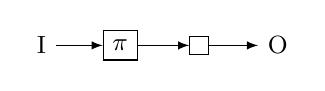
\begin{tikzpicture}[auto,>=latex]
  \node[] (input) {\code{I}};
  \node[block, right of=input] (pi) {$\pi$};
  \node[block, right of=pi] (distinct) {$\distinct$};
  \node[right of=distinct] (output) {\code{O}};
  \draw[->] (input) -- (pi);
  \draw[->] (pi) -- (distinct);
  \draw[->] (distinct) -- (output);
\end{tikzpicture}
&
\parbox[b][][t]{\commentsize}{
$\pi(i)[y] \defn
\sum_{x \in i, x|_c = y} i[x]$ \\
$x|_c$ is projection on column $c$ of the tuple $x$ \\
$\pi$ is linear; $\ispositive(\pi)$ %, \zpp{\pi}$.
}
\\ \hline
Filtering &
\begin{lstlisting}[language=SQL]
SELECT * FROM I
WHERE p(I.c)
\end{lstlisting}
&
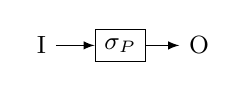
\begin{tikzpicture}[auto,>=latex]
  \node[] (input) {\code{I}};
  \node[block, right of=input] (map) {$\sigma_P$};
  \node[right of=map] (output) {\code{O}};
  \draw[->] (input) -- (map);
  \draw[->] (map) -- (output);
\end{tikzpicture}
&
\parbox[b][][t]{\commentsize}{
$\sigma_P(m)[x] \defn \left\{
\begin{array}{ll}
  m[x] & \mbox{ if } P(x) \\
  0 & \mbox{ otherwise } \\
\end{array}
\right.$ \\
$P: A \rightarrow \B$ is a predicate. \\
$\sigma_P$ is linear; $\ispositive(\sigma_P)$ % \zpp{\sigma_P}$.
}
% \\ \hline
%Selection &
%\begin{lstlisting}[language=SQL]
%SELECT DISTINCT f(I.c, ...)
%FROM I
%\end{lstlisting}
%&
%\begin{tikzpicture}[auto,>=latex]
%  \node[] (input) {\code{I}};
%  \node[block, right of=input, node distance=1.5cm] (map) {$\mbox{map}(f)$};
%  \node[block, right of=map, node distance=1.5cm] (distinct) {$\distinct$};
%  \node[right of=distinct, node distance=1.5cm] (output) {\code{O}};
%  \draw[->] (input) -- (map);
%  \draw[->] (map) -- (distinct);
%  \draw[->] (distinct) -- (output);
%\end{tikzpicture}
%&
%\parbox[b][][t]{\commentsize}{
%For a function $f$ \\
%$\map(f)$ is linear, \\
%$\ispositive(\map(f)), \zpp{\map(f)}$
%}.
\\ \hline
\parbox[b][][t]{1cm}{
Cartesian \\
product} &
\begin{lstlisting}[language=SQL]
SELECT I1.*, I2.*
FROM I1, I2
\end{lstlisting}
&
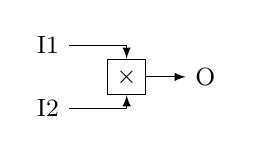
\begin{tikzpicture}[auto,>=latex]
  \node[] (i1) {\code{I1}};
  \node[below of=i1, node distance=.4cm] (midway) {};
  \node[below of=midway, node distance=.4cm] (i2) {\code{I2}};
  \node[block, right of=midway] (prod) {$\times$};
  \node[right of=prod] (output) {\code{O}};
  \draw[->] (i1) -| (prod);
  \draw[->] (i2) -| (prod);
  \draw[->] (prod) -- (output);
\end{tikzpicture}
&
\parbox[b][][t]{\commentsize}{
$(a \times b)((x,y)) \defn a[x] \times b[y]$. \\
$\times$ is bilinear, $\ispositive(\times)$ % , \zpp{\times}$.
}
\\ \hline
Equi-join &
\begin{lstlisting}[language=SQL]
SELECT I1.*, I2.*
FROM I1 JOIN I2
ON I1.c1 = I2.c2
\end{lstlisting}
&
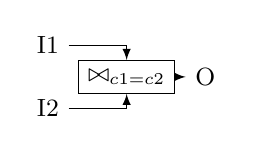
\begin{tikzpicture}[auto,>=latex]
  \node[] (i1) {\code{I1}};
  \node[below of=i1, node distance=.4cm] (midway) {};
  \node[below of=midway, node distance=.4cm] (i2) {\code{I2}};
  \node[block, right of=midway] (prod) {$\bowtie_{c1 = c2}$};
  \node[right of=prod] (output) {\code{O}};
  \draw[->] (i1) -| (prod);
  \draw[->] (i2) -| (prod);
  \draw[->] (prod) -- (output);
\end{tikzpicture}
&
\parbox[b][][t]{\commentsize}{
$(a \bowtie b)((x,y)) \defn a[x] \times b[y] \\
\mbox{ if } x|_{c1} = y|_{c2}$. \\
$\bowtie$ is bilinear, $\ispositive(\bowtie)$ %, \zpp{\bowtie}$.
}
\\ \hline
Intersection &
\begin{lstlisting}[language=SQL]
(SELECT * FROM I1)
INTERSECT
(SELECT * FROM I2)
\end{lstlisting}
&
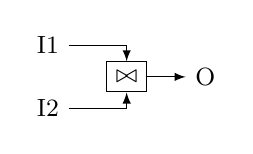
\begin{tikzpicture}[auto,>=latex]
  \node[] (i1) {\code{I1}};
  \node[below of=i1, node distance=.4cm] (midway) {};
  \node[below of=midway, node distance=.4cm] (i2) {\code{I2}};
  \node[block, right of=midway] (prod) {$\bowtie$};
  \node[right of=prod] (output) {\code{O}};
  \draw[->] (i1) -| (prod);
  \draw[->] (i2) -| (prod);
  \draw[->] (prod) -- (output);
\end{tikzpicture}
&
Special case of equi-join when both relations have the same schema.
 \\ \hline
Difference &
\begin{lstlisting}[language=SQL]
SELECT * FROM I1
EXCEPT
SELECT * FROM I2
\end{lstlisting}
&
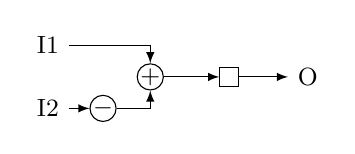
\begin{tikzpicture}[auto,>=latex, node distance=.7cm]
  \node[] (i1) {\code{I1}};
  \node[below of=i1, node distance=.4cm] (midway) {};
  \node[below of=midway, node distance=.4cm] (i2) {\code{I2}};
  \node[block, shape=circle, inner sep=0in, right of=i2] (m) {$-$};
  \node[block, right of=midway, shape=circle, inner sep=0in, node distance=1.3cm] (plus) {$+$};
  \node[block, right of=plus, node distance=1cm] (distinct) {$\distinct$};
  \node[right of=distinct, node distance=1cm] (output) {\code{O}};
  \draw[->] (i1) -| (plus);
  \draw[->] (i2) -- (m);
  \draw[->] (m) -| (plus);
  \draw[->] (plus) -- (distinct);
  \draw[->] (distinct) -- (output);
\end{tikzpicture}
&
$\distinct$ removes elements with negative weights from the result.
\\ \hline
\end{tabular}
\end{table*}


The translation is fairly straightforward, but many operators require
the application of a $\distinct$ \textbf{to produce sets}.
For example, $a \cup b = \distinct(a + b)$, $a \setminus b =
\distinct(a - b)$, $(a \times b)((x,y)) = a[x] \times b[y]$.
%\paragraph{Correctness of the \dbsp implementations}\label{sec:correctness}
%
%A relational query $Q$ that transforms
%a set $V$ into a set $U$ is implemented by a \dbsp computation $Q'$ on
%\zrs.  The correctness of the implementation requires the following
%diagram to commute:
%
%\begin{center}
%\begin{tikzpicture}
%  \node[] (V) {$V$};
%  \node[below of=V] (VZ) {$VZ$};
%  \node[right of=V, node distance=2cm] (U) {$U$};
%  \node[below of=U] (UZ) {$UZ$};
%  \draw[->] (V) -- node (f) [below] {$Q$} (U);
%  \draw[->] (V) --  node (s) [left] {tozset}(VZ);
%  \draw[->] (VZ) -- node (f) [above] {$Q'$} (UZ);
%  \draw[->] (UZ) -- node (d) [right] {toset} (U);
%\end{tikzpicture}
%\end{center}
%
%(The correctness of
%this implementation is predicated on $Q'$'s inputs being
%sets, an invariant which needs to be maintained by the environment.)
%The ``$\mbox{toset}$'' and ``$\mbox{tozset}$'' functions convert sets to \zrs and
%vice-versa, in the expected way:
%
%$\mbox{toset}: \Z[A] \to 2^A$ is defined as $\mbox{toset}(m) \defn \cup_{x \in \distinct(m)} \{ x \}$.
%
%$\mbox{tozset}: 2^A \to \Z[A]$ is defined as $\mbox{tozset}(s) \defn \sum_{x \in s} 1 \cdot x$.
%
%All standard algebraic properties
%of the relational operators can be used to optimize circuits
%(they can even be applied to queries before building the circuits).
%
Notice that the use of the $\distinct$ operator allows \dbsp to model
the \emph{full relational algebra}, including set difference (and not
just the positive fragment).

Prior work (e.g., Proposition 6.13 in~\cite{green-tcs11}) has shown
how some invocations of $\distinct$ can be eliminated from query plans
without changing the query semantics; we will see that incremental
versions of $\distinct$ operators incur significant space costs.

\begin{proposition}\label{prop-distinct-delay}
Let $Q$ be one of the following \zrs operators: filtering $\sigma$,
join $\bowtie$, or Cartesian product $\times$.
Then we have $\forall i \in \Z[I], \ispositive(i) \Rightarrow Q(\distinct(i)) = \distinct(Q(i))$.
\end{proposition}

\begin{comment}
\noindent
\begin{tabular}{m{3.5cm}m{.5cm}m{3.5cm}}
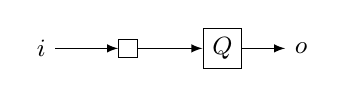
\begin{tikzpicture}[auto,>=latex]
  \node[] (input) {$i$};
  \node[block, right of=input, node distance=1.1cm] (distinct) {$\distinct$};
  \node[block, right of=distinct, node distance=1.2cm] (q) {$Q$};
  \node[right of=q] (output)  {$o$};
  \draw[->] (input) -- (distinct);
  \draw[->] (distinct) -- (q);
  \draw[->] (q) -- (output);
\end{tikzpicture}
&
$\cong$
&
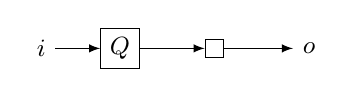
\begin{tikzpicture}[auto,>=latex]
  \node[] (input) {$i$};
  \node[block, right of=input] (q) {$Q$};
  \node[block, right of=q, node distance=1.2cm] (distinct1) {$\distinct$};
  \node[right of=distinct1, node distance=1.2cm] (output)  {$o$};
  \draw[->] (input) -- (q);
  \draw[->] (q) -- (distinct1);
  \draw[->] (distinct1) -- (output);
\end{tikzpicture}
\end{tabular}

This rule allows us to delay the application of $\distinct$.
\end{comment}

\begin{proposition}\label{prop-distinct-once}
Let $Q$ be one of the following \zrs operators: filtering $\sigma$,
projection $\pi$, map($f$)\footnote{Technically, map (applying a user-defined
function to each row) is not relational.},
addition $+$, join $\bowtie$, or
Cartesian product $\times$.
Then we have $\ispositive(i) \Rightarrow \distinct(Q(\distinct(i))) = \distinct(Q(i))$.
\end{proposition}

\begin{comment}
\noindent
\begin{tabular}{m{6.5cm}m{.5cm}}
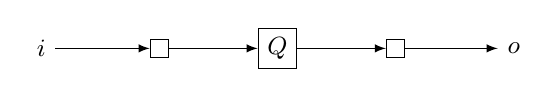
\begin{tikzpicture}[auto,>=latex]
  \node[] (input) {$i$};
  \node[block, right of=input, node distance=1.5cm] (distinct) {$\distinct$};
  \node[block, right of=distinct, node distance=1.5cm] (q) {$Q$};
  \node[block, right of=q, node distance=1.5cm] (distinct1) {$\distinct$};
  \node[right of=distinct1, node distance=1.5cm] (output)  {$o$};
  \draw[->] (input) -- (distinct);
  \draw[->] (distinct) -- (q);
  \draw[->] (q) -- (distinct1);
  \draw[->] (distinct1) -- (output);
\end{tikzpicture}
&
$\cong$ \\
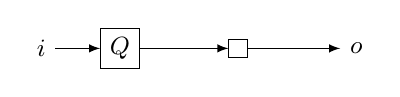
\begin{tikzpicture}[auto,>=latex]
  \node[] (input) {$i$};
  \node[block, right of=input] (q) {$Q$};
  \node[block, right of=q, node distance=1.5cm] (distinct1) {$\distinct$};
  \node[right of=distinct1, node distance=1.5cm] (output)  {$o$};
  \draw[->] (input) -- (q);
  \draw[->] (q) -- (distinct1);
  \draw[->] (distinct1) -- (output);
\end{tikzpicture}
\end{tabular}
\end{comment}

These properties allow us to ``consolidate'' distinct operators by performing
one $\distinct$ at the end of a chain of computations.

\subsection{Incremental view maintenance}

Let us consider a relational query $Q$ defining a view $V$.  To create
a circuit that maintains incrementally $V$ we apply the following
mechanical steps:

\begin{algorithm}[incremental view maintenance]\label{algorithm-inc}\quad
\begin{enumerate}[nosep, leftmargin=\parindent]
    \item Translate $Q$ into a circuit using the rules in Table~\ref{tab:relational}.
    \item Apply $\distinct$ elimination rules (\ref{prop-distinct-delay}, \ref{prop-distinct-once}) until convergence\footnote{The
    order in which the rules are applied does not matter, since the algorithm is
    confluent: it always produces the same final result.}.
    \item Lift the whole circuit, by applying Proposition~\ref{prop:distributivity},
    converting it to a circuit operating on streams.
    \item Incrementalize the whole circuit ``surrounding'' it with $\I$ and $\D$.
    \item Apply the chain rule
    from Proposition~\ref{prop-inc-properties} recursively on the query structure
    to obtain an incremental implementation.
\end{enumerate}
\end{algorithm}

This algorithm is deterministic and its running time
is proportional to the number of operators in the query.
Step (2) generates an equivalent circuit, with possibly fewer
$\distinct$ operators.  Step (3) yields a circuit that consumes a
\emph{stream} of complete database snapshots and outputs a stream of
complete view snapshots. Step (4) yields a circuit that consumes a
stream of \emph{database changes} and outputs a stream of \emph{view
changes}; however, the internal operation of the circuit is
non-incremental, as it rebuilds the complete database using
integration operators.  Step (5) incrementalizes the circuit by
replacing each primitive operator with its incremental version.

Most of the operators that appear in the circuits in
Table~\ref{tab:relational} are linear, and thus have very efficient
incremental versions (we discuss complexity in
\refsec{sec:complexity}).  A notable exception is $\distinct$.  The
next proposition shows that the incremental version of $\distinct$ is
also efficient, and it can be computed by doing work proportional to
the size of the input change:

\begin{proposition}\label{prop-inc_distinct}
The following circuit implements $\inc{(\lift{\distinct})}$:
\begin{tabular}{m{3.5cm}m{.0cm}m{5cm}}
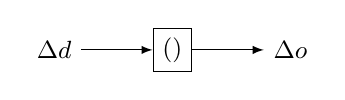
\begin{tikzpicture}[auto,node distance=1.5cm,>=latex]
    \node[] (input) {$\Delta d$};
    \node[block, right of=input] (d) {$\inc{(\lift{\distinct})}$};
    \node[right of=d] (output) {$\Delta o$};
    \draw[->] (input) -- (d);
    \draw[->] (d) -- (output);
\end{tikzpicture} &
$\cong$ &
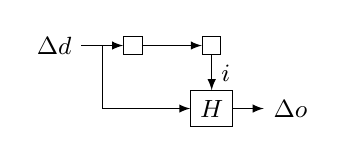
\begin{tikzpicture}[>=latex]
    \node[] (input) {$\Delta d$};
    \node[block, right of=input] (I) {$\I$};
    \node[block, right of=I] (z) {$\zm$};
    \node[block, below of=z, node distance=.8cm] (H) {$\lift{H}$};
    \node[right of=H] (output) {$\Delta o$};
    \draw[->] (input) -- node (mid) {} (I);
    \draw[->] (I) -- (z);
    \draw[->] (mid.center) |- (H);
    \draw[->] (z) -- node (i) [right] {$i$} (H);
    \draw[->] (H) -- (output);
\end{tikzpicture}
\end{tabular}

\noindent where $H: \Z[A] \times \Z[A] \to \Z[A]$ is defined as: \\
$$
H(i, d)[x] \defn
\begin{cases}
-1 & \mbox{if } i[x] > 0 \mbox{ and } (i + d)[x] \leq 0 \\
1  & \mbox{if } i[x] \leq 0 \mbox{ and } (i + d)[x] > 0 \\
0  & \mbox{otherwise} \\
\end{cases}
$$
\end{proposition}

Here is the intuition why $\distinct$ is efficiently
incrementalizable: the only elements that can appear in the output of
$\inc{(\lift{\distinct})}$ must have changed in the input.  So the
size of the output change cannot be bigger than the size of the input
change.  In the diagram above, $i$ is the previous version of the
integral of all changes, i.e., the full \zr whose $\distinct$ value is
being computed.  The function $H$ detects whether the weight of
an element in $i$ is changing sign (positive to negative or
vice-versa) when adding a new delta $d$.

%\refsec{sec:relational-example} shows a concrete example of a relational query converted
%into a circuit and then incrementalized using Algorithm~\ref{algorithm-inc}.

\subsection{Complexity of incremental circuits}\label{sec:complexity}

Incremental circuits are efficient.  We evaluate the cost of a circuit
while processing the $t$-th input change.  Even if $Q$ is a pure
function, $\inc{Q}$ is actually a streaming system, with internal
state.  This state is stored entirely in the delay operators $\zm$,
some of which appear in $\I$ and $\D$ operators.  The result produced
by $\inc{Q}$ on the $t$-th input depends in general not only on the
new $t$-th input, but also on all prior inputs it has received.

We argue that each operator in the incremental version of a circuit is
efficient in terms of work and space.  We make the standard IVM
assumption that the input changes \emph{of each operator} are small:
$|\Delta DB[t]| \ll |DB[t]| = |(\I(\Delta DB))[t]|$.

An unoptimized incremental operator $\inc{Q} = \D \circ Q \circ \I$
evaluates query $Q$ on the whole database $DB$, the integral of the input stream:
$DB = \I(\Delta DB)$; hence its time complexity  is the same as that of the non-incremental
evaluation of $Q$.  In addition, each of the $\I$ and $\D$ operators uses $O(|DB[t]|)$ memory.

Step (5) of the incrementalization algorithm applies the optimizations described in \secref{sec:incremental};
these reduce the time complexity of each operator to be a function of $O(|\Delta DB[t]|)$.
For example, Theorem~\ref{linear}, allows evaluating $\inc{S}$, where $S$ is a
linear operator, in time $O(|\Delta DB[t]|)$.  The $\I$
operator can also be evaluated in $O(|\Delta DB[t]|)$ time, because
all values that appear in the output of $\I(\Delta DB)[t]$ must be present in
current input change $\Delta DB[t]$.  Similarly, while the $\distinct$ operator is not
linear, $\inc{(\lift{\distinct})}$ can also be evaluated in $O(|\Delta DB[t]|)$ according to
Proposition~\ref{prop-inc_distinct}.  Bilinear operators, including join, can be
evaluated in time $O(|DB[t]| \times |\Delta DB[t]|)$, which is a factor of $|DB[t] / \Delta DB[t]|$
better than full re-evaluation.

The space complexity of linear operators is 0 (zero), since they store no
data persistently.  The space complexity of operators such as $\inc{(\lift{\distinct})}$,
$\inc{(\lift{\bowtie})}$, $\I$, and $\D$ is $O(|DB[t]|)$.  They need
to store their input or output relations in full.

\subsubsection{IVM query plans and optimality}

Let us look again at what we achieved using
Algorithm~\ref{algorithm-inc}.  A relational algebra query can be
implemented by multiple plans, each with a different data-dependent
cost\footnote{The optimal plan depends not only on the query, but also
  on the data.}.  The input of Algorithm~\ref{algorithm-inc} is a
(relational), non-incremental query plan, produced by a query planner.
The algorithm produces an incremental plan that is ``similar'' to the
input plan.

Standard query planners use cost-based heuristics and data statistics
to optimize plans.  A generic IVM planner does not have this luxury,
since the plan must be generated \emph{before} any data has been fed
to the database.  Nevertheless, all standard query optimization
techniques, perhaps based on historical statistics, can be used to
generate the query plan that is supplied to
Algorithm~\ref{algorithm-inc}.  The question of optimality in the
context of IVM plan is a much more difficult topic than optimization
of ad-hoc queries, since the chosen IVM plan will execute for
\emph{all future database updates}.

Moreover, since incremental computations maintain internal state, it
follows that incremental plans cannot be simply changed in-flight,
like we can change ad-hoc queries based on current data statistics:
deploying a new plan requires in general constructing its internal
state, which is produced by entire history of prior updates.
Fortunately, there is a trivial, but somewhat expensive, recipe for
installing a new incremental plan: feed the entire current state of
the database, as one big change.

\subsection{Relational Query Example}\label{sec:relational-example}

We apply the IVM algorithm~\ref{algorithm-inc} to a concrete
relational SQL query:
\begin{lstlisting}[language=SQL,basicstyle=\small]
CREATE VIEW v AS
SELECT DISTINCT a.x, b.y FROM (
     SELECT t1.x, t1.id FROM t1 WHERE t1.a > 2
) a JOIN (
     SELECT t2.id, t2.y FROM t2 WHERE t2.s > 5
) b ON a.id = b.id
\end{lstlisting}

Step 1: Create a \dbsp circuit to represent this query using the
translation rules from Table~\ref{tab:relational}; notice that
this circuit is essentially a dataflow implementation of the query.
(Notice that the query asks for \code{SELECT DISTINCT}, so there is a
$\distinct$ operator after $\sigma$):

\noindent
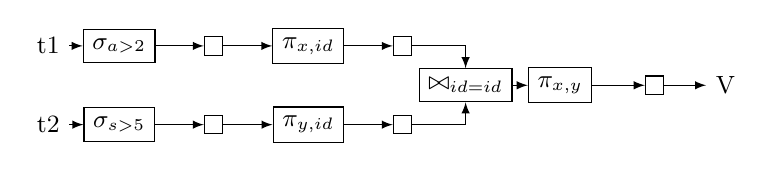
\begin{tikzpicture}[node distance=1.2cm,>=latex]
    \node[] (t1) {\code{t1}};
    \node[block, right of=t1, node distance=.9cm] (s1) {$\sigma_{a > 2}$};
    \node[block, right of=s1] (d1) {$\distinct$};
    \node[block, right of=d1] (p1) {$\pi_{x, id}$};
    \node[block, right of=p1] (d11) {$\distinct$};
    \node[below of=t1, node distance=1cm] (t2) {\code{t2}};
    \node[block, right of=t2, node distance=.9cm] (s2) {$\sigma_{s > 5}$};
    \node[block, right of=s2] (d2) {$\distinct$};
    \node[block, right of=d2] (p2) {$\pi_{y, id}$};
    \node[block, right of=p2] (d21) {$\distinct$};
    \node[below of=d11, node distance=.5cm] (mid) {};
    \node[block, right of=mid, node distance=.8cm] (j) {$\bowtie_{id = id}$};
    \node[block, right of=j] (p) {$\pi_{x, y}$};
    \node[block, right of=p] (d) {$\distinct$};
    \node[right of=d, node distance=.9cm] (V) {\code{V}};
    \draw[->] (t1) -- (s1);
    \draw[->] (s1) -- (d1);
    \draw[->] (d1) -- (p1);
    \draw[->] (p1) -- (d11);
    \draw[->] (t2) -- (s2);
    \draw[->] (s2) -- (d2);
    \draw[->] (d2) -- (p2);
    \draw[->] (p2) -- (d21);
    \draw[->] (d11) -| (j);
    \draw[->] (d21) -| (j);
    \draw[->] (j) -- (p);
    \draw[->] (p) -- (d);
    \draw[->] (d) -- (V);
\end{tikzpicture}

Step 2: apply the rules to eliminate $\distinct$ operators.
First from Proposition~\ref{prop-distinct-once}:

\noindent
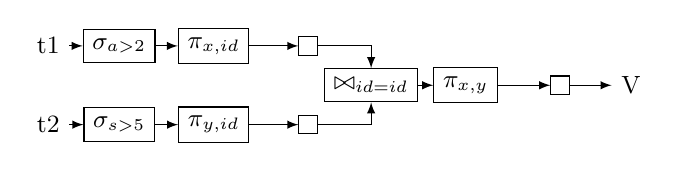
\begin{tikzpicture}[node distance=1.2cm,>=latex]
    \node[] (t1) {\code{t1}};
    \node[block, right of=t1, node distance=.9cm] (s1) {$\sigma_{a > 2}$};
    \node[block, right of=s1] (p1) {$\pi_{x, id}$};
    \node[block, right of=p1] (d11) {$\distinct$};
    \node[below of=t1, node distance=1cm] (t2) {\code{t2}};
    \node[block, right of=t2, node distance=.9cm] (s2) {$\sigma_{s > 5}$};
    \node[block, right of=s2] (p2) {$\pi_{y, id}$};
    \node[block, right of=p2] (d21) {$\distinct$};
    \node[below of=d11, node distance=.5cm] (mid) {};
    \node[block, right of=mid, node distance=.8cm] (j) {$\bowtie_{id = id}$};
    \node[block, right of=j] (p) {$\pi_{x, y}$};
    \node[block, right of=p] (d) {$\distinct$};
    \node[right of=d, node distance=.9cm] (V) {\code{V}};
    \draw[->] (t1) -- (s1);
    \draw[->] (s1) -- (p1);
    \draw[->] (p1) -- (d11);
    \draw[->] (t2) -- (s2);
    \draw[->] (s2) -- (p2);
    \draw[->] (p2) -- (d21);
    \draw[->] (d11) -| (j);
    \draw[->] (d21) -| (j);
    \draw[->] (j) -- (p);
    \draw[->] (p) -- (d);
    \draw[->] (d) -- (V);
\end{tikzpicture}

\noindent The rule from Proposition~\ref{prop-distinct-delay} gives
(from now on we omit the subscripts to save space):

\noindent
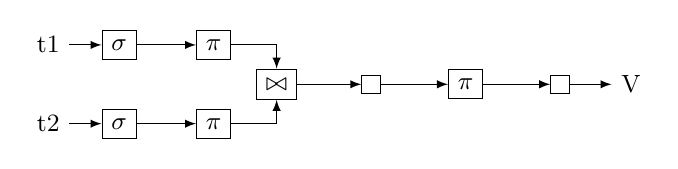
\begin{tikzpicture}[node distance=1.2cm,>=latex]
    \node[] (t1) {\code{t1}};
    \node[block, right of=t1, node distance=.9cm] (s1) {$\sigma$};
    \node[block, right of=s1] (p1) {$\pi$};
    \node[below of=t1, node distance=1cm] (t2) {\code{t2}};
    \node[block, right of=t2, node distance=.9cm] (s2) {$\sigma$};
    \node[block, right of=s2] (p2) {$\pi$};
    \node[below of=p1, node distance=.5cm] (mid) {};
    \node[block, right of=mid, node distance=.8cm] (j) {$\bowtie$};
    \node[block, right of=j] (d0) {$\distinct$};
    \node[block, right of=d0] (p) {$\pi$};
    \node[block, right of=p] (d) {$\distinct$};
    \node[right of=d, node distance=.9cm] (V) {\code{V}};
    \draw[->] (t1) -- (s1);
    \draw[->] (s1) -- (p1);
    \draw[->] (t2) -- (s2);
    \draw[->] (s2) -- (p2);
    \draw[->] (p1) -| (j);
    \draw[->] (p2) -| (j);
    \draw[->] (j) -- (d0);
    \draw[->] (d0) -- (p);
    \draw[->] (p) -- (d);
    \draw[->] (d) -- (V);
\end{tikzpicture}

\noindent And again~\ref{prop-distinct-once}:

\noindent
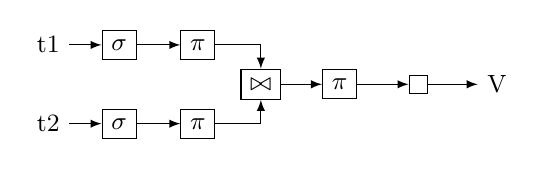
\begin{tikzpicture}[node distance=1cm,>=latex]
    \node[] (t1) {\code{t1}};
    \node[block, right of=t1, node distance=.9cm] (s1) {$\sigma$};
    \node[block, right of=s1] (p1) {$\pi$};
    \node[below of=t1, node distance=1cm] (t2) {\code{t2}};
    \node[block, right of=t2, node distance=.9cm] (s2) {$\sigma$};
    \node[block, right of=s2] (p2) {$\pi$};
    \node[below of=p1, node distance=.5cm] (mid) {};
    \node[block, right of=mid, node distance=.8cm] (j) {$\bowtie$};
    \node[block, right of=j] (p) {$\pi$};
    \node[block, right of=p] (d) {$\distinct$};
    \node[right of=d, node distance=1cm] (V) {\code{V}};
    \draw[->] (t1) -- (s1);
    \draw[->] (s1) -- (p1);
    \draw[->] (t2) -- (s2);
    \draw[->] (s2) -- (p2);
    \draw[->] (p1) -| (j);
    \draw[->] (p2) -| (j);
    \draw[->] (j) -- (p);
    \draw[->] (p) -- (d);
    \draw[->] (d) -- (V);
\end{tikzpicture}

At this point no more $\distinct$ elimination rules can be applied.

Step 3: we lift the circuit using distributivity of composition over
lifting (Proposition~\ref{prop:distributivity}); we obtain a circuit
that computes over streams, i.e., for each new input pair of relations
\code{t1} and \code{t2} it will produce an output view \code{V}:

\noindent
\begin{tikzpicture}[node distance=1cm,>=latex]
    \node[] (t1) {\code{t1}};
    \node[block, right of=t1, node distance=.9cm] (s1) {$\lift{\sigma}$};
    \node[block, right of=s1] (p1) {$\lift{\pi}$};
    \node[below of=t1, node distance=1cm] (t2) {\code{t2}};
    \node[block, right of=t2, node distance=.9cm] (s2) {$\lift{\sigma}$};
    \node[block, right of=s2] (p2) {$\lift{\pi}$};
    \node[below of=p1, node distance=.5cm] (mid) {};
    \node[block, right of=mid, node distance=.8cm] (j) {$\lift{\bowtie}$};
    \node[block, right of=j] (p) {$\lift{\pi}$};
    \node[block, right of=p, node distance=1.2cm] (d) {$\lift{\distinct}$};
    \node[right of=d] (V) {\code{V}};
    \draw[->] (t1) -- (s1);
    \draw[->] (s1) -- (p1);
    \draw[->] (t2) -- (s2);
    \draw[->] (s2) -- (p2);
    \draw[->] (p1) -| (j);
    \draw[->] (p2) -| (j);
    \draw[->] (j) -- (p);
    \draw[->] (p) -- (d);
    \draw[->] (d) -- (V);
\end{tikzpicture}

Step 4: incrementalize circuit, obtaining a circuit that computes over changes;
this circuit receives changes to relations \code{t1} and \code{t2} and for each
such change it produces the corresponding change in the output view \code{V}:

\noindent
\begin{tikzpicture}[node distance=1cm,>=latex]
    \node[] (t1) {$\Delta$\code{t1}};
    \node[block, right of=t1, node distance=.8cm] (I1) {$\I$};
    \node[block, right of=I1, node distance=.9cm] (s1) {$\lift{\sigma}$};
    \node[block, right of=s1] (p1) {$\lift{\pi}$};
    \node[below of=t1, node distance=1cm] (t2) {$\Delta$\code{t2}};
    \node[block, right of=t2, node distance=.8cm] (I2) {$\I$};
    \node[block, right of=I2, node distance=.9cm] (s2) {$\lift{\sigma}$};
    \node[block, right of=s2] (p2) {$\lift{\pi}$};
    \node[below of=p1, node distance=.5cm] (mid) {};
    \node[block, right of=mid, node distance=.7cm] (j) {$\lift{\bowtie}$};
    \node[block, right of=j] (p) {$\lift{\pi}$};
    \node[block, right of=p, node distance=1.2cm] (d) {$\lift{\distinct}$};
    \node[block, right of=d, node distance=1.1cm] (D) {$\D$};
    \node[right of=D, node distance=.8cm] (V) {$\Delta$\code{V}};
    \draw[->] (t1) -- (I1);
    \draw[->] (I1) -- (s1);
    \draw[->] (s1) -- (p1);
    \draw[->] (t2) -- (I2);
    \draw[->] (I2) -- (s2);
    \draw[->] (s2) -- (p2);
    \draw[->] (p1) -| (j);
    \draw[->] (p2) -| (j);
    \draw[->] (j) -- (p);
    \draw[->] (p) -- (d);
    \draw[->] (d) -- (D);
    \draw[->] (D) -- (V);
\end{tikzpicture}

Step 5: apply the chain rule to rewrite the circuit as a composition of incremental operators;

\noindent
\begin{tikzpicture}[node distance=1.6cm,>=latex]
    \node[] (t1) {$\Delta$\code{t1}};
    \node[block, right of=t1, node distance=1.2cm] (s1) {$\inc{(\lift{\sigma})}$};
    \node[block, right of=s1] (p1) {$\inc{(\lift{\pi})}$};
    \node[below of=t1, node distance=1.2cm] (t2) {$\Delta$\code{t2}};
    \node[block, right of=t2, node distance=1.2cm] (s2) {$\inc{(\lift{\sigma})}$};
    \node[block, right of=s2] (p2) {$\inc{(\lift{\pi})}$};
    \node[below of=p1, node distance=.6cm] (mid) {};
    \node[block, right of=mid, node distance=.8cm] (j) {$\inc{(\lift{\bowtie})}$};
    \node[block, right of=j] (p) {$\inc{(\lift{\pi})}$};
    \node[block, right of=p] (d) {$\inc{(\lift{\distinct})}$};
    \node[right of=d, node distance=1.2cm] (V) {$\Delta$\code{V}};.8
    \draw[->] (t1) -- (s1);
    \draw[->] (s1) -- (p1);
    \draw[->] (t2) -- (s2);
    \draw[->] (s2) -- (p2);
    \draw[->] (p1) -| (j);
    \draw[->] (p2) -| (j);
    \draw[->] (j) -- (p);
    \draw[->] (p) -- (d);
    \draw[->] (d) -- (V);
\end{tikzpicture}

Use the linearity of $\sigma$ and $\pi$ to simplify this circuit (notice that
all linear operators no longer have a $\inc{\cdot}$):

\noindent
\begin{tikzpicture}[node distance=1cm,>=latex]
    \node[] (t1) {$\Delta$\code{t1}};
    \node[block, right of=t1, node distance=1cm] (s1) {$\lift{\sigma}$};
    \node[block, right of=s1] (p1) {$\lift{\pi}$};
    \node[below of=t1, node distance=1.2cm] (t2) {$\Delta$\code{t2}};
    \node[block, right of=t2, node distance=1cm] (s2) {$\lift{\sigma}$};
    \node[block, right of=s2] (p2) {$\lift{\pi}$};
    \node[below of=p1, node distance=.6cm] (mid) {};
    \node[block, right of=mid, node distance=.8cm] (j) {$\inc{(\lift{\bowtie})}$};
    \node[block, right of=j] (p) {$\lift{\pi}$};
    \node[block, right of=p, node distance=1.2cm] (d) {$\inc{(\lift{\distinct})}$};
    \node[right of=d, node distance=1.3cm] (V) {$\Delta$\code{V}};
    \draw[->] (t1) -- (s1);
    \draw[->] (s1) -- (p1);
    \draw[->] (t2) -- (s2);
    \draw[->] (s2) -- (p2);
    \draw[->] (p1) -| (j);
    \draw[->] (p2) -| (j);
    \draw[->] (j) -- (p);
    \draw[->] (p) -- (d);
    \draw[->] (d) -- (V);
\end{tikzpicture}

Finally, replace the incremental join using the formula for bilinear operators
(Theorem~\ref{bilinear}),
and the incremental $\distinct$ (Proposition~\ref{prop-inc_distinct}),
obtaining the following circuit:

\noindent
\begin{tikzpicture}[node distance=.8cm,>=latex]
    \node[] (t1) {$\Delta$\code{t1}};
    \node[block, right of=t1] (s1) {$\lift{\sigma}$};
    \node[block, right of=s1] (p1) {$\lift{\pi}$};
    \node[below of=t1, node distance=.8cm] (t2) {$\Delta$\code{t2}};
    \node[block, right of=t2] (s2) {$\lift{\sigma}$};
    \node[block, right of=s2] (p2) {$\lift{\pi}$};

    % join expansion
      \node[block, right of=p1] (jI1) {$\I$};
      \node[block, right of=p2] (jI2) {$\I$};
      \draw[->] (p1) -- (jI1);
      \draw[->] (p2) -- (jI2);
      \node[block, right of=jI2] (ZI2) {$\zm$};
      \draw[->] (jI2) -- (ZI2);
      \node[block, right of=jI1] (DI1) {$\lift\bowtie$};
      \node[block, right of=ZI2, node distance=1cm] (DI2) {$\lift\bowtie$};
      \draw[->] (jI1) -- (DI1);
      \draw[->] (ZI2) -- (DI2);
      \node[block, circle, above of=DI2, inner sep=0cm] (sum) {$+$};
      \draw[->] (DI1) -- (sum);
      \draw[->] (DI2) -- (sum);
      \draw[->] (p1) -- (DI2);
      \draw[->] (p2) -- (DI1);

    \node[block, right of=sum] (p) {$\lift{\pi}$};
    \draw[->] (sum) -- (p);
    \node[block, right of=p] (Id) {$\I$};
    \node[block, right of=Id] (zd) {$\zm$};
    \node[block, below of=zd] (H) {$\lift{H}$};
    \node[right of=H] (V) {$\Delta$\code{V}};
    \draw[->] (t1) -- (s1);
    \draw[->] (s1) -- (p1);
    \draw[->] (t2) -- (s2);
    \draw[->] (s2) -- (p2);
    \draw[->] (p) -- node (tapp) {} (Id);
    \draw[->] (Id) -- (zd);
    \draw[->] (zd) -- (H);
    \draw[->] (tapp.center) |- (H);
    \draw[->] (H) -- (V);
\end{tikzpicture}

Notice that the resulting circuit contains three integration
operations: two from the join, and one from the $\distinct$.  It also
contains two join operators.  However, the work performed by each
operator for each new input is proportional to the size of the change.


\section{Recursive queries}\label{sec:recursion}

Recursive queries are very useful in a many applications.
For example, graph algorithms such as graph reachability
or transitive closure are naturally expressed using recursive queries.

We introduce two simple \dbsp stream operators that are used for
expressing recursive query evaluation.  These operators allow us
to build circuits implementing looping constructs, which
are used to iterate computations until a fixed-point is reached.

\begin{definition}\label{def:zae}
We say that a stream $s \in \stream{A}$ is \defined{zero almost-everywhere} if it has a finite
number of non-zero values, i.e., there exists a time $t_0 \in \N$
s.t. $\forall t \geq t_0 . s[t] = 0$.
\noindent Denote the set of streams that are zero almost everywhere
by $\streamf{A} \subset \stream{A}$.
\end{definition}

\paragraph{Stream introduction}

The delta function (named from the Dirac delta function) $\delta_0 : A \rightarrow \stream{A}$
produces a stream from a scalar value:
$$\delta_0(v)[t] \defn \left\{
\begin{array}{ll}
  v & \mbox{if } t = 0 \\
  0_A & \mbox{ otherwise}
\end{array}
\right.
$$
\ifstreamexamples
For example, $\delta_0(5)$ is the stream $\sv{5 0 0 0 0}$.
\fi

\begin{comment}
Here is a diagram showing a $\delta_0$ operator; note that the input is a scalar value,
while the output is a stream:

\begin{tikzpicture}[auto,node distance=1cm,>=latex]
    \node[] (input) {$i$};
    \node[block, right of=input] (delta) {$\delta_0$};
    \node[right of=delta] (output) {$o$};
    \draw[->] (input) -- (delta);
    \draw[->] (delta) -- (output);
\end{tikzpicture}
\end{comment}

\paragraph{Stream elimination}

We define the function $\int : \streamf{A} \rightarrow
A$, over streams that are zero almost everywhere, as
$\int(s) \defn \sum_{t \geq 0} s[t]$.
$\int$ is closely related to $\I$; if $\I$ is the
indefinite (discrete) integral, $\int$ is the definite (discrete) integral on the
interval $0 - \infty$.  For example, $\int(\sv{1 2 3 0 0}) = 6$.

For many classes of queries (including relational and Datalog queries
given below) the $\int$ operator can be ``approximated'' without loss
of precision by integrating until the first 0 value encountered.

\begin{comment}
Here is a diagram using the $\int$ operator; note that  the result it
produces is a scalar, and not a stream:

\begin{tikzpicture}[auto,node distance=1cm,>=latex]
    \node[] (input) {$i$};
    \node[block, right of=input] (S) {$\int$};
    \node[right of=S] (output) {$o$};
    \draw[->] (input) -- (S);
    \draw[->] (S) -- (output);
\end{tikzpicture}
\end{comment}

%$\delta_0$ is the left inverse of $\int$, i.e.: $\int \circ \; \delta_0 = \id_A$.
\begin{proposition}
$\delta_0$ and $\int$ are LTI.
\end{proposition}

\paragraph{Nested time domains}

So far we have used a tacit assumption that ``time'' is common for all
streams in a program.  For example, when we add two streams,
we assume that they use the same ``clock'' for the time dimension.
However, the $\delta_0$ operator creates a stream with a ``new'', independent time
dimension.  We require \emph{well-formed circuits}
to ``insulate'' such
nested time domains by ``bracketing'' them between a $\delta_0$
and an $\int$ operator:

\begin{center}
\begin{tikzpicture}[auto,node distance=1cm,>=latex]
    \node[] (input) {$i$};
    \node[block, right of=input] (delta) {$\delta_0$};
    \node[block, right of=delta] (f) {$Q$};
    \draw[->] (input) -- (delta);
    \draw[->>] (delta) -- (f);

    \node[block, right of=f] (S) {$\int$};
    \node[right of=S] (output) {$o$};
    \draw[->>] (f) -- (S);
    \draw[->] (S) -- (output);
\end{tikzpicture}
\end{center}

In this circuit the arrows with double
heads denote stream values, while the simple arrow denote scalar values\footnote{We only use this convention in this diagram;
in general the type of an arrow can be inferred from the type
of its source node.}.  $Q$ is a streaming operator, but the entire circuit is a scalar function.

Algorithm~\ref{algorithm-rec} below, which translates recursive queries to
\dbsp circuits, always produces well-formed circuits.
%\begin{proposition}
%If $Q$ is time-invariant, the circuit above has the zero-preservation
%property: $\zpp{\int \circ\; Q \circ \delta_o}$.
%\end{proposition}

\subsection{Implementing recursive queries}\label{sec:datalog}

We describe the implementation of recursive queries in \dbsp for
stratified Datalog.
In general, a recursive Datalog program defines a set of
mutually recursive relations $O_1,..,O_n$ as an equation
$(O_1,..,O_n)=R(I_1,..,I_m, O_1,..,O_n)$, where $I_1,..,I_m$ are
input relations and $R$ is a relational (non-recursive) query.

We describe the algorithm for
the simpler case of a single-input, single-output query\footnote{The general case
in the companion technical report~\anonymize{\cite{tr}} is only
slightly more involved.}.  The input of our algorithm is a Datalog query of the form
$O = R(I, O)$, where $R$ is a relational, non-recursive query,
producing a set as a result, but whose output $O$ is also an input.
The output of the algorithm is a \dbsp circuit which evaluates this
recursive query producing output $O$ when given the input $I$.  Here we build
a non-incremental circuit, which evaluates the Datalog query;
in \refsec{sec:nested} we derive the incremental version
of this circuit.

\begin{algorithm}[recursive queries]\label{algorithm-rec}
\noindent
\begin{enumerate}[nosep, leftmargin=\parindent]
\item Implement the non-recursive relational query $R$ as described in
    \secref{sec:relational} and Table~\ref{tab:relational}; this produces
    an acyclic circuit whose inputs and outputs are a \zrs:
    \begin{center}
    \begin{tikzpicture}[auto,>=latex]
      \node[] (I) {\code{I}};
      \node[below of=I, node distance=.5cm] (O) {\code{O}};
      \node[block, right of=I] (R) {$R$};
      \node[right of=R] (o) {\code{O}};
      \draw[->] (I) -- (R);
      \draw[->] (O) -| (R);
      \draw[->] (R) -- (o);
    \end{tikzpicture}
    \end{center}

\item Lift this circuit to operate on streams:
    \begin{center}
    \begin{tikzpicture}[auto,>=latex]
      \node[] (I) {\code{I}};
      \node[below of=I, node distance=.5cm] (O) {\code{O}};
      \node[block, right of=I] (R) {$\lift R$};
      \node[right of=R] (o) {\code{O}};
      \draw[->] (I) -- (R);
      \draw[->] (O) -| (R);
      \draw[->] (R) -- (o);
    \end{tikzpicture}
    \end{center}
  We construct $\lift{R}$ by lifting each operator of the circuit individually
  according to Proposition~\ref{prop:distributivity}.

\item Build a cycle, connecting the output to the corresponding
recursive input via a delay:

 \begin{center}
\begin{tikzpicture}[auto,>=latex, node distance=.8cm]
  \node[] (I) {\code{I}};
  \node[block, right of=I] (R) {$\lift R$};
  \node[right of=R, node distance=1.5cm] (O) {\code{O}};
  \node[block, below of=R, node distance=.7cm] (z) {$\zm$};
  \draw[->] (I) -- (R);
  \draw[->] (R) -- node(o) {} (O);
  \draw[->] (o) |- (z);
  \draw[->] (z) -- (R);
 \end{tikzpicture}
 \end{center}
\item ``Bracket'' the circuit in $\I$ and $\D$ nodes, and then in $\delta_0$ and $\int$:

\begin{center}
\begin{tikzpicture}[auto,>=latex, node distance=.8cm]
  \node[] (Iinput) {\code{I}};
  \node[block, right of=Iinput] (ID) {$\delta_0$};
  \node[block, right of=ID] (II) {$\I$};
  \node[block, right of=II] (f) {$\lift{R}$};
  \node[block, right of=f, node distance=1.5cm] (D) {$\D$};
  \node[block, right of=D] (S) {$\int$};
  \node[right of=S] (output)  {\code{O}};
  \draw[->] (Iinput) -- (ID);
  \draw[->] (ID) -- (II);
  \draw[->] (II) -- (f);
  \draw[->] (f) -- node (o) {} (D);
  \draw[->] (D) -- (S);
  \draw[->] (S) -- (output);
  \node[block, below of=f, node distance=.7cm] (z) {$\zm$};
  \draw[->] (o) |- (z);
  \draw[->] (z) -- (f);
\end{tikzpicture}
\end{center}
\end{enumerate}
\end{algorithm}

We argue that the cycle inside this circuit computes iteratively the fixed point of $R$.
The $\D$ operator yields the set of new Datalog facts (changes) computed by each iteration of the loop.
When the set of new facts becomes empty, the fixed point has been reached:

\begin{theorem}[Recursion correctness]\label{theorem:recursion}
If $\isset(\code{I})$, the output of the circuit above is
the relation $\code{O}$ as defined by the Datalog semantics of given program
$R$ as a function of the input relation \code{I}.
\end{theorem}
\label{proof-recursion}
%\begin{proof}
%Let us compute the contents of the $o$ stream, produced at the output
%of $R$.  We will show that this stream is composed
%of increasing approximations of the value of \code{O}.
%
%Define the following one-argument function: $S(x) = \lambda x . R(\code{I}, x)$.
%Notice that the left input of the $\lift{R}$ block is a constant stream
%with the value \code{I}.  Due to the stratified nature of the language,
%we must have $\ispositive(S)$, so $\forall x . S(x) \geq x$.
%We get the following system of equations:
%$$
%\begin{aligned}
%o[0] =& S(0) \\
%o[t] =& S(o[t-1]) \\
%\end{aligned}
%$$
%So, by induction on $t$ we have $o[t] = S^t(0)$, where by
%$S^t$ we mean $\underbrace{S \circ S \circ \ldots \circ S}_{t}$.
%$S$ is monotone; thus, if there is a time $k$ such that $S^k(0) = S^{k+1}(0)$, we have
%$\forall j \in \N . S^{k+j}(0) = S^k(0)$.  Applying a $\D$ to this stream
%will then produce a stream that is zero almost everywhere, and integrating
%this result will return the last distinct value in the stream $o$.
%
%This is essentially the definition of the semantics of a recursive Datalog relation:
%$\code{O} = \fix{x}{R(\code{I}, x)}$.
%\end{proof}

Note that if the query $R$ computes over unbounded data domains (e.g.,
using integers with arithmetic), this construction does not guarantee
that at runtime a fixed point is reached.  But if a program does converge, the
above construction will find the least fixed point.

In fact, this circuit implements the standard \defined{na\"{\i}ve evaluation}
algorithm (e.g., see Algorithm~1 in \cite{greco-sldm15}).
Notice that the inner part of the circuit is the incremental
form of another circuit, since it is sandwiched between $\I$ and $\D$ operators.
Using the cycle rule of Proposition~\ref{prop-inc-properties} we can rewrite this circuit as:
%
\begin{equation}
\begin{aligned}
\label{eq:seminaive}
\begin{tikzpicture}[auto,>=latex]
  \node[] (Iinput) {\code{I}};
  \node[block, right of=Iinput] (Idelta) {$\delta_0$};
  \node[block, right of=Idelta] (f) {$\inc{(\lift{R})}$};
  \node[block, right of=f, node distance=1.5cm] (S) {$\int$};
  \node[right of=S] (output)  {\code{O}};
  \node[block, below of=f, node distance=.7cm] (z) {$\zm$};
  \draw[->] (Iinput) -- (Idelta);
  \draw[->] (f) -- node (o) {} (S);
  \draw[->] (S) -- (output);
  \draw[->] (o) |- (z);
  \draw[->] (z) -- (f);
  \draw[->] (Idelta) -- (f);
\end{tikzpicture}
\end{aligned}
\end{equation}

This circuit implements \defined{semi-na\"{\i}ve evaluation}
(Algorithm~2 from~\cite{greco-sldm15}).  We have just proven the
correctness of semi-na\"{\i}ve evaluation as an immediate consequence
of the cycle rule!

%In \refsec{sec:recursive-example} we show a concrete example, applying Algorithm~\ref{algorithm-rec}
%to a recursive query computing the transitive closure of a graph.

\section{Nested streams}\label{sec:nested}

\subsection{Creating and destroying streams}\label{sec:stream-intro-elim}

We introduce two new stream operators that are instrumental in
expressing recursive query evaluation.  These operators allow us
to build circuits implementing looping constructs, which
are used to iterate computations until a fixed-point is reached.

\subsubsection{Stream introduction}\label{sec:stream-introduction}

\begin{definition}[Dirac delta]
The delta function (named from the Dirac delta function) $\delta_0 : A \rightarrow \stream{A}$
produces a stream from a scalar value.
The output stream is produced as follows from the input scalar:

$$\delta_0(v)[t] \defn \left\{
\begin{array}{ll}
  v & \mbox{if } t = 0 \\
  0_A & \mbox{ otherwise}
\end{array}
\right.
$$
\end{definition}

Here is a diagram showing a $\delta_0$ operator; note that the input is a scalar value,
while the output is a stream:

\begin{center}
\begin{tikzpicture}[auto,node distance=1cm,>=latex]
    \node[] (input) {$i$};
    \node[block, right of=input] (delta) {$\delta_0$};
    \node[right of=delta] (output) {$o$};
    \draw[->] (input) -- (delta);
    \draw[->] (delta) -- (output);
\end{tikzpicture}
\end{center}

For example, $\delta_0(5)$ is the stream $\sv{5 0 0 0 0}$.

\subsubsection{Stream elimination}\label{sec:stream-elimination}

Recall that $\streamf{A}$ was defined in Definition~\ref{def:zae} to be the set of
$A$-streams over a group $A$ that are zero almost everywhere.

\begin{definition}[indefinite integral]
We define a function $\int : \streamf{A} \rightarrow
A$ as $\int(s) \defn \sum_{t \geq 0} s[t]$.
\end{definition}

$\int$ is closely related to $\I$; if $\I$ is the
indefinite integral, $\int$ is the definite integral on the
interval $0 - \infty$.   Unlike $\I$
$\int$ produces a scalar value, the ``last'' distinct value that would
appear in the stream produced by $\I$.
For example $\int(\cut{\id}{4}) = 0 + 1 + 2 + 3 = 6$, because
$\I(\cut{\id}{4}) = \sv{0 1 3 6 6}$.

An alternative definition for $\int$ for all streams $\stream{A}$
would extend the set $A$ with an ``infinite'':
$\overline{A} \defn A \cup \{ \top \}$, and define $\int{s} \defn
\top$ for streams that are not zero a.e., $s \in \stream{A} \setminus \streamf{A}$.

Here is a diagrams showing the $\int$ operator; note that  the result it
produces is a scalar, and not a stream:

\begin{center}
\begin{tikzpicture}[auto,node distance=1cm,>=latex]
    \node[] (input) {$i$};
    \node[block, right of=input] (S) {$\int$};
    \node[right of=S] (output) {$o$};
    \draw[->] (input) -- (S);
    \draw[->] (S) -- (output);
\end{tikzpicture}
\end{center}

$\delta_0$ is the left inverse of $\int$, i.e., the
following equation holds: $\int \circ \;\delta_0 = \id_A$.

\subsubsection{The $E$ and $X$ operators}

The composition $\I \circ \delta_0$ is frequently used, so we
will give it a name, denoting it by $E: A \to \stream{A}$, $E \defn \I \circ \delta_0$.

\begin{center}
\begin{tabular}{m{2cm}m{.5cm}m{4cm}}
\begin{tikzpicture}[auto,>=latex]
  \node[] (input) {};
  \node[block, right of=input] (E) {$E$};
  \node[right of=E] (output) {};
  \draw[->] (input) -- (E);
  \draw[->] (E) -- (output);
\end{tikzpicture} &
$\defn$ &
\begin{tikzpicture}[auto,>=latex]
  \node[] (input) {};
  \node[block, right of=input] (delta) {$\delta_0$};
  \node[block, right of=delta] (i) {$\I$};
  \node[right of=i] (output) {};
  \draw[->] (input) -- (delta);
  \draw[->] (delta) -- (i);
  \draw[->] (i) -- (output);
\end{tikzpicture}
\end{tabular}
\end{center}

Notice that the output of the $E$ operator is a constant infinite stream, consisting the scalar
value at the input.  $E(5) = \sv{5 5 5 5 5}$.

Similarly, we denote by $X: \stream{A} \to A$ the combination $X \defn \int \circ \D$.

\begin{center}
\begin{tabular}{m{2cm}m{.5cm}m{4cm}}
\begin{tikzpicture}[auto,>=latex]
  \node[] (input) {};
  \node[block, right of=input] (X) {$X$};
  \node[right of=X] (output) {};
  \draw[->] (input) -- (X);
  \draw[->] (E) -- (output);
\end{tikzpicture} &
$\defn$ &
\begin{tikzpicture}[auto,>=latex]
  \node[] (input) {};
  \node[block, right of=input] (D) {$\D$};
  \node[block, right of=D] (i) {$\int$};
  \node[right of=i] (output) {};
  \draw[->] (input) -- (D);
  \draw[->] (D) -- (i);
  \draw[->] (i) -- (output);
\end{tikzpicture}
\end{tabular}
\end{center}

\begin{proposition}
For a monotone stream $o \in \stream{A}$ we have
$X(o) = \lim_{n \to \infty} o[n]$, if the limit exists.
\end{proposition}
\begin{proof}
$X(\cut{o}{n}) = (\int \circ \D)(\cut{o}{n}) = o[0] + (o[1] - o[0]) + \ldots + (o[n] - o[n-1]) = o(n)$.
The result follows by taking limits on both sides.
\end{proof}
\mihai{This looks almost right, but it is not.}

Clearly, $E$ is the left-inverse of $X$.

\begin{proposition}
$\delta_0$, $\int$, $E$, and $X$ are LTI.
\end{proposition}
\begin{proof}
The proof is easy using simple algebraic manipulation of the definitions of these operators.
\end{proof}

\subsubsection{Time domains}\label{sec:time-domains}

So far we had the tacit assumption that ``time'' is common for all
streams in a program.  For example, when we add two streams,
we assume that they use the same ``clock'' for the time dimension.
However, the $\delta_0$ operator creates a streams with a ``new'', independent time
dimension.  In Section~\ref{sec:wfc} we will define some well-formed circuit
construction rules that will ensure that such time domains are always ``insulated'',
by requiring each diagram that starts with a $\delta_0$ operator
to end with a corresponding $\int$ operator:

\begin{center}
\begin{tikzpicture}[auto,node distance=1cm,>=latex]
    \node[] (input) {$i$};
    \node[block, right of=input] (delta) {$\delta_0$};
    \node[block, right of=delta] (f) {$Q$};
    \draw[->] (input) -- (delta);
    \draw[->] (delta) -- (f);

    \node[block, right of=f] (S) {$\int$};
    \node[right of=S] (output) {$o$};
    \draw[->] (f) -- (S);
    \draw[->] (S) -- (output);
\end{tikzpicture}
\end{center}


\begin{proposition}
If $Q$ is time-invariant, the circuit above has the zero-preservation
property: $\zpp{\int \circ\; Q \circ \delta_o}$.
\end{proposition}
\begin{proof}
  This follows from the fact that all three operators preserve zeros, and thus so
  does their composition.
\end{proof}

\subsection{Streams of streams}\label{sec:nested}

\subsubsection{Defining nested streams}

Since all streams we work with are defined over abelian groups
and streams themselves form an abelian group, as pointed in Section~\ref{sec:abelianstreams},
it follows that we can naturally define streams of streams.
$\stream{\stream{A}} = \N \rightarrow (\N \rightarrow A)$.  This construction
can be iterated, but our applications do not require more than
two-level nesting.  Box-and-arrow diagrams can be used equally to
depict functions computing on nested streams; in this case an
arrow represent a stream where each value is another stream.

\newcommand{\ssa}[1]{
\setsepchar{ }
\readlist\arg{#1}
\begin{bmatrix}
   \begin{array}{ccccccc}
        {[} & \arg[1] & \arg[2] & \arg[3] & \arg[4] & \cdots & {]} \\
        {[} & \arg[5] & \arg[6] & \arg[7] & \arg[8] & \cdots & {]} \\
        {[} & \arg[9] & \arg[10] & \arg[11] & \arg[12] & \cdots & {]} \\
        {[} & \arg[13] & \arg[14] & \arg[15] & \arg[16] & \cdots & {]} \\
        \multicolumn{7}{c}{\vdots}
   \end{array}
\end{bmatrix}
}

Equivalently, a nested stream in $\stream{\stream{A}}$ is a value in
$\N \times \N \to A$, i.e., a ``matrix''
with an infinite number of rows, where each row is a stream.
For example, we can depict the nested stream
$i \in \stream{\stream{\N}}$ defined by $i[t_0][t_1] = t_0 + 2 t_1$ as:
$$ i = \ssa{0 1 2 3 2 3 4 5 4 5 6 7 6 7 8 9} $$

\noindent ($t_0$ is the column index, and $t_1$ is the row index).

\subsubsection{Lifting stream operators}

We have originally defined lifting (Section~\ref{sec:lifting}) for scalar functions.
We can generalize lifting to apply to stream operators as well.  Consider a
stream operator $S: \stream{A} \to \stream{B}$.  We define $\lift{S}: \stream{\stream{A}}
\to \stream{\stream{B}}$ as: $(\lift{S}(s))[t_0][t_1] \defn S(s[t_0])[t_1], \forall t_0, t_1 \in
\N$.  Alternatively, we can write $(\lift{S})(s) = S \circ s$.

In particular, a scalar function $f: A \rightarrow B$ can be can lifted twice to
produce an operator between streams of streams: $\lift{\lift{f}}: \stream{\stream{A}}
\rightarrow \stream{\stream{B}}$.

Lifting twice a scalar function computes on elements of the matrix pointwise:

$$(\lift{\lift{(x \mapsto x \bmod 2)}})(i) =
  \ssa{0 1 0 1 0 1 0 1 0 1 0 1 0 1 0 1}
$$

$\zm$ delays the rows of the matrix:

$$\zm(i) = \ssa{0 0 0 0 0 1 2 3 2 3 4 5 4 5 6 7}$$

\noindent while its lifted counterpart delays each column of the matrix:

$$(\lift{\zm})(i) = \ssa{0 0 1 2 0 2 3 4 0 4 5 6 0 6 7 8}$$

We can also apply both operators, and they commute:

$$(\lift{\zm})(\zm(i)) = \zm((\lift{\zm})(i)) = \ssa{0 0 0 0 0 0 1 2 0 2 3 4 0 4 5 6}$$

Similarly, we can apply $\D$ to nested streams $\D : \stream{\stream{A}} \to
\stream{\stream{A}}$, computing on rows of the matrix:

$$\D(i) = \ssa{0 1 2 3 2 2 2 2 2 2 2 2 2 2 2 2}$$

\noindent while $\lift{\D} : \stream{\stream{A}} \to \stream{\stream{A}}$
computes on the columns:

$$(\lift{\D})(i) = \ssa{0 1 1 1 2 1 1 1 4 1 1 1 6 1 1 1}$$

Similarly, we can apply both differentiation operators in sequence:

$$(\D(\lift{\D}))(i) = \ssa{0 1 1 1 2 0 0 0 2 0 0 0 2 0 0 0}$$

\begin{comment}
\subsubsection{Matrix representations of nested streams}\label{sec:matrix-picture}

Similar to the vector graphical representations from \refsec{sec:vector-picture},
we can use a graphical representation of a nested stream $s$:

$\mtrx{0 0 0 0}$

The four rectangles correspond to the following expressions:
$$
\begin{aligned}
\I(\lift{\I}(s))[t_0-1][t_1-1] = \I(\zm(\lift{\I}(\lift{\zm})))[t_0][t_1] =& \mtrx{1 0 0 0} \\
\I(s)[t_0][t_1-1] = \I(\zm(s))[t_0][t_1] =& \mtrx{0 1 0 0} \\
\lift{\I(s)}[t_0-1][t_1] = \lift{\I(\lift{\zm})}(s)[t_0][t_1] =& \mtrx{0 0 1 0} \\
s[t_0][t_1] =& \mtrx{0 0 0 1}.
\end{aligned}
$$

Lifting a vector we obtain a matrix, e.g.:
$\lift{\strm{1 0}} = \mtrx{1 0 1 0}$.

Consider a bilinear scalar operator $\times$.  Let us expand the following expression:
$\inc{(\lift{(\inc{(\lift{(a \times b)})})})}$.

In Section~\ref{sec:vector-picture} we expanded the inner term
$$
\begin{aligned}
\inc{(\lift{a \times b})} = &\matmult{\strm{1 0}}{\strm{0 1}} \\
&\matmult{\strm{0 1}}{\strm{1 0}} \\
&\matmult{\strm{0 1}}{\strm{0 1}}
\end{aligned}
$$

Lifting this term again we get:

$$
\begin{aligned}
\lift{(\inc{(\lift{(a \times b)})})} =&
\matmult{\mtrx{1 0 1 0}}{\mtrx{0 1 0 1}} +\\
&\matmult{\mtrx{0 1 0 1}}{\mtrx{1 0 1 0}} +\\
&\matmult{\mtrx{0 1 0 1}}{\mtrx{0 1 0 1}}
\end{aligned}
$$

And now we apply incrementalize this again, by expanding each
term into 3 other terms and regrouping due to distributivity of $\times$ over addition (bilinearity):

$$
\begin{aligned}
\inc{(\lift{(\inc{(\lift{(a \times b)})})})} = \\
%
\matmult{\mtrx{1 0 0 0}}{\mtrx{0 0 0 1}} +
\matmult{\mtrx{0 0 1 0}}{\mtrx{0 1 0 0}} + \\
\matmult{\mtrx{0 0 1 0}}{\mtrx{0 0 0 1}} + \\
%
\matmult{\mtrx{0 1 0 0}}{\mtrx{0 0 1 0}} +
\matmult{\mtrx{0 0 0 1}}{\mtrx{1 0 0 0}} +\\
\matmult{\mtrx{0 0 0 1}}{\mtrx{0 0 1 0}} +\\
%
\matmult{\mtrx{0 1 0 0}}{\mtrx{0 0 0 1}} +
\matmult{\mtrx{0 0 0 1}}{\mtrx{0 1 0 0}} + \\
\matmult{\mtrx{0 0 0 1}}{\mtrx{0 0 0 1}} = \\
%
\matmult{\mtrx{1 1 1 1}}{\mtrx{0 0 0 1}} +
\matmult{\mtrx{0 0 1 1}}{\mtrx{0 1 0 0}} + \\
\matmult{\mtrx{0 0 0 1}}{\mtrx{1 0 0 0}} +
\matmult{\mtrx{0 1 0 1}}{\mtrx{0 0 1 9}}.
\end{aligned}
$$
\end{comment}

\subsubsection{Strict operators on nested streams}

In order to show that operators defined using feedback are well-defined on
nested streams we need to extend the notion of strict operators from Section~\ref{sec:causal}.

We define a partial order over timestamps: $(i_0, i_1)
\leq (t_0, t_1)$ iff $i_0 \leq t_0$ and $i_1 \leq t_1$.  We extend the
definition of strictness for operators over nested streams: a stream operator
$F: \stream{\stream{A}} \to \stream{\stream{B}}$ is strict if for any $s, s' \in
\stream{\stream{A}}$ and all times $t, i \in \N \times \N$ we have $\forall i <
t, s[i] = s'[i]$ implies $F(s)[t] = F(s')[t]$.
Proposition~\ref{prop-unique-fix} holds for this notion of strictness, i.e., the fixed point operator $\fix{\alpha}{F(\alpha)}$ is well defined for a strict operator $F$.
\mihai{Should write down this proof.}

\begin{proposition}\label{prop-liftz}
The operator $\lift{\zm}: \stream{\stream{A}} \to \stream{\stream{A}}$ is strict.
\end{proposition}

The $\I$ operator on $\stream{\stream{A}}$ is well-defined: it operates on rows
of the matrix, treating each row as a single value:

$$\I(i) = \ssa{0 1 2 3 2 4 6 8 6 9 12 15 12 16 20 24}$$

With this extended notion of strictness we have that the lifted integration operator
is also well-defined: $\lift{\I}: \stream{\stream{A}} \to \stream{\stream{A}}.$
This operator integrates each column of the stream matrix:

$$(\lift{\I})(i) = \ssa{0 1 3 6 2 5 9 14 4 9 15 22 6 13 21 30}$$

Notice the following commutativity properties for integration and differentiation
on nested streams: $\I \circ (\lift{\I}) = (\lift{\I}) \circ \I$ and
$\D \circ (\lift{\D}) = (\lift{\D}) \circ \D$.

\begin{comment}
\subsection{Multidimensional integrals and derivatives}

We now define a generalized form of the $\I$ and $\D$ operators to compute on
streams nested arbitrarily deep.
We define these operators inductively on the structure of the type $A$ of elements that
they compute on, as follows:

\begin{definition}[Generalized integration] The generalized integration operator
for values of type $A$ is denoted by $\I_A: A \to A$ and is defined as follows:
$$
\begin{aligned}
\I_A &\defn \id & \mbox{ when $A$ is a scalar type}, \\
\I_{\stream{A}} &\defn \I \circ \lift{\I_A} & \mbox{otherwise.}
\end{aligned}
$$
\end{definition}


\begin{definition}[Generalized differentiation] The generalized differentiation operator
for values of type $A$ is denoted by $\D_A: A \to A$ and is defined as follows:
$$
\begin{aligned}
\D_A &\defn \id & \mbox{when $A$ is a scalar type,} \\
\D_{\stream{A}} &\defn \lift{\D_A} \circ \D &\mbox{otherwise}
\end{aligned}
$$
\end{definition}


$$\I_{\stream{\stream{\N}}}(i) = ((\lift{\I})(\I))(i)= \ssa{0 1 3 6 2 6 12 20 6 15 27 42 12 28 48 72}$$


Recall the definition we gave for the incremental version of an operator $Q: \stream{A} \to \stream{B}$
in Section~\ref{sec:incremental}: $\inc{Q} = \D \circ Q \circ \I$.  We want to generalize this
definition so that it applies to arbitrary functions on streams of various nesting depths.

\begin{definition}
The incremental version of a function $f: A \to B$ is a function $\inc{f}: A \to B$ defined as
$\inc{f} \defn \D_B \circ f \circ \I_A$.
\end{definition}

Clearly, this definition generalizes the one we gave before.

Let us compute the incremental version of a twice-lifted scalar operator:
$\inc{(\lift{\lift{f}})} = \D \circ (\lift{\D}) \circ
(\lift{\lift{f}}) \circ (\lift{\I}) \circ \I$.

This definition allows us to talk about the incremental forms of
the two special stream creation and destruction operators from Section~\ref{sec:stream-intro-elim}:

$\inc{\delta_0} = \D \circ \delta_0$.

$\inc{\int} = \int \circ \I$.

\subsubsection{Properties of the generalized incremental transform}

All properties from Theorem~\ref{prop-inc-properties} hold true with our
generalized definition, replacing the integrals and differentials
with their generalized versions.  In addition we have:

\begin{enumerate}
\item $\inc{(\lift{Q})} = \D \circ \lift{(\inc{Q})} \circ \I$.
\item $\inc{(\lift{\I})} = \lift{\I}$ since $\lift{\I}$ is linear, being
the lifted version of a linear operator.
\item $\inc{(\lift{\D})} = \lift{\D}$ since $\lift{\D}$ is linear.
\item $\inc{(\lift{+})} = \lift{+} = +$.
\item $\inc{(\lift{\zm})} = \lift{\zm}$ since $\lift{\zm}$ is linear.
\end{enumerate}
\end{comment}

\subsubsection{Lifted cycles}

\begin{proposition}[Lifting cycles]
\label{prop-lift-cycle}
For a binary, causal $T$ we have:
$$\lift{(\lambda s. \fix{\alpha}{T(s,\zm(\alpha)}))} = \lambda s. \fix{\alpha}{(\lift{T})(s,(\lift{\zm})(\alpha))}$$
\noindent i.e., lifting a circuit containing a ``cycle'' can be accomplished by
lifting all operators independently.
\end{proposition}
\begin{proof}
Consider a stream of streams $a =[a_0, a_1, a_2, \cdots ] \in \stream{\stream{A}}$
(where each $a_i \in \stream{A}$).  The statement to prove becomes:
$$
\lift{(\lambda s. \fix{\alpha}{T(s,\zm(\alpha)}))}(a) =
\fix{\alpha}{(\lift{T})(a,(\lift{\zm})(\alpha))}
$$
This follows if we show that the value defined as:
$$
\beta = \lift{(\lambda s. \fix{\alpha}{T(s,\zm(\alpha)}))}(a)
$$
satisfies
$$
\beta = (\lift{T})(a,(\lift{\zm})(\beta))
$$
Now, expanding the definition of lifting a function:
$$
\begin{aligned}
\lift{(\lambda s. \fix{\alpha}{T(s,\zm(\alpha)}))}(a) &\defn
\lift{(\lambda s. \fix{\alpha}{T(x,\zm(\alpha)}))}([a_0,a_1,\cdots]) \\
&\defn [\fix{\alpha}{T(a_0,\zm(\alpha))}, \fix{\alpha}{T(a_1,\zm(\alpha))}, \cdots] \\
&= [\alpha_0,\alpha_1,\alpha_2,\cdots]
\end{aligned}
$$
where, $\forall i . \alpha_i$ is the unique solution of the equation
$\alpha_i=T(a_i,\zm(\alpha_i))$.
Finally, for $\beta =[\alpha_0,\alpha_1,\cdots]$ we have
$$
(\lift{T})([a_0,a_1,\ldots],(\lift{\zm})(\beta))
= [T(a_0,\zm(\alpha_0)),T(a_1,\zm(\alpha_1)), \ldots]
$$
which finishes the proof.
\end{proof}

Proposition~\ref{prop-lift-cycle} gives us the tool to lift whole circuits.
For example, we have:

\begin{center}
\begin{tabular}{m{2cm}m{.5cm}m{4cm}}
\begin{tikzpicture}[>=latex]
  \node[] (input) {$i$};
  \node[block, right of=input] (I) {$\lift{\I}$};
  \node[right of=I] (output)  {$o$};
  \draw[->] (input) -- (I);
  \draw[->] (I) -- (output);
\end{tikzpicture}
& $\cong$ &
\begin{tikzpicture}[>=latex]
  \node[] (input) {$i$};
  \node[block, circle, right of=input, inner sep=0cm] (p) {$+$};
  \node[right of=p, node distance=1.5cm] (output)  {$o$};
  \node[block, below of=p, node distance=.8cm] (z) {$\lift{\zm}$};
  \draw[->] (input) -- (p);
  \draw[->] (p) -- node (mid) {} (output);
  \draw[->] (z) -- (p);
  \draw[->] (mid.center) |- (z);
\end{tikzpicture}
\end{tabular}
\end{center}

As another example, consider the following circuit $T: A \to B$ that represents a \emph{scalar} function:

\begin{center}
\begin{tikzpicture}[auto,>=latex]
  \node[] (input) {$i$};
  \node[block, right of=input] (delta) {$\delta_0$};
  \node[block, shape=circle, right of=delta, inner sep=0in] (plus) {$+$};
  \node[block, right of=plus] (f) {$\lift{Q}$};
  \node[block, right of=f, node distance=1.5cm] (S) {$\int$};
  \node[right of=S] (output)  {$o$};
  \draw[->] (input) -- (delta);
  \draw[->] (delta) -- (plus);
  \draw[->] (plus) -- (f);
  \draw[->] (f) -- node (o) {} (S);
  \draw[->] (S) -- (output);
  \node[block, below of=f] (z) {$\zm$};
  \draw[->] (o) |- (z);
  \draw[->] (z) -| (plus);
\end{tikzpicture}
\end{center}

Since this circuit represents a scalar function, it can be lifted like
any other scalar function to create a stream computation\footnote{Notice that
+ is not shown lifted in this circuit, since there is in fact a + operator for any
type, and we have that $\lift({+_A}) = +_{\stream{A}}$}:

\begin{center}
\begin{tikzpicture}[auto,>=latex]
  \node[] (input) {$i$};
  \node[block, right of=input] (delta) {$\lift{\delta_0}$};
  \node[block, shape=circle, right of=delta, inner sep=0in] (plus) {$+$};
  \node[block, right of=plus] (f) {$\lift{\lift{Q}}$};
  \node[block, right of=f, node distance=1.5cm] (S) {$\lift{\int}$};
  \node[right of=S] (output)  {$o$};
  \draw[->] (input) -- (delta);
  \draw[->] (delta) -- (plus);
  \draw[->] (plus) -- (f);
  \draw[->] (f) -- node (o) {} (S);
  \draw[->] (S) -- (output);
  \node[block, below of=f] (z) {$\lift{\zm}$};
  \draw[->] (o) |- (z);
  \draw[->] (z) -| (plus);
\end{tikzpicture}
\end{center}

\subsection{Fixed-point computations}

\begin{theorem}
Given a scalar operator $Q: A \rightarrow A$, the output stream $o$ computed by the
following diagram (using the lifted version of $Q$) is given by $\forall t \in \N . o[t] = Q^{t+1}(i)$, where $k$ is the composition
of $Q$ with itself $k$ times.

\begin{center}
\begin{tikzpicture}[auto,>=latex]
  \node[] (input) {$i$};
  \node[block, right of=input] (delta) {$\delta_0$};
  \node[block, shape=circle, right of=delta, inner sep=0in] (plus) {$+$};
  \node[block, right of=plus, node distance=1cm] (q) {$\lift{Q}$};
  \node[right of=q, node distance=2cm] (output)  {$o$};
  \draw[->] (input) -- (delta);
  \draw[->] (delta) -- (plus);
  \draw[->] (plus) -- (q);
  \draw[->] (q) -- node (o) {} (output);
  \node[block, below of=q] (z) {$\zm$};
  \draw[->] (o) |- (z);
  \draw[->] (z) -| (plus);
\end{tikzpicture}
\end{center}
\end{theorem}
\begin{proof}
  Let us compute $o[t]$.  We have that $o[0] =
  Q(\delta_0(i)[0] + 0) = Q(i)$.  $o[1] =
  Q(o[0] + \delta_0(i)[1]) =
  Q(Q(i) + 0) = Q^2(i)$.  We can prove by induction
  over $t$ that $o[t] = Q^{t+1}(i)$.
\end{proof}

\textbf{Observation}: in this circuit the ``plus'' operator behaves as an \code{if}, selecting between
the base case and the inductive case in a recursive definition.
This is because the left input contains a single non-zero
element ($i$), in the first position, while the bottom input starts with a 0.


\begin{comment}
\subsection{Flattening nested streams}

We now introduce two constructions that allow converting a stream of ``bounded'' streams into
a simple stream.

\paragraph{Time-indexed streams}

We first introduce an operator that labels each element of a stream $\stream{A}$ with a ``time'' value.
This is defined by the following circuit:

\begin{tikzpicture}[auto,>=latex]
  \node[] (input) {$s$};
  \node[block, right of=input, node distance=1.5cm] (c) {$\lift{(x \mapsto 1)}$};
  \node[block, right of=c, node distance=1.5cm] (I) {$\I$};
  \node[below of=I] (below) {};
  \node[block, right of=below] (p) {$\pair{\cdot}{\cdot}$};
  \node[right of=p] (output) {$o$};
  \draw[->] (input) -- node (tap) {} (c);
  \draw[->] (c) -- (I);
  \draw[->] (I) -| (p);
  \draw[->] (tap) |- (p);
  \draw[->] (p) -- (output);
\end{tikzpicture}

The circuits starts from a stream $s$, then generates a stream of constant values $1 \in \N$ for
each element of $s$, which it then integrates and pairs with the input stream.  Given a stream $\sv{a b c d e}$
this produces the stream $\sv{\pair{a}{1} \pair{b}{2} \pair{c}{3} \pair{d}{4} \pair{e}{5}}$.

\paragraph{Truncated finite streams}

Given a stream that is zero almost everywhere $s \in \streamf{A}$, let us define an operator
that returns the ``interesting'' prefix of the stream, containing all non-zero elements:
$\trunc{\cdot}: \streamf{A} \rightarrow A[\N]$.  The result of this operator is a ``vector''
having a finite length.

\paragraph{Flattened streams}

Consider a stream of streams where each inner stream is zero almost everywhere: $\stream{\streamf{A}}$.
The we define the $\mbox{flat}$ operator $\mbox{flat}: \stream{\streamf{A}} \rightarrow \stream{A \times N}$.

\end{comment}

%\section{Additional query languages}\label{sec:extensions}

In this section we describe several query models that go behind stratified Datalog
and show how they can be implemented in \dbsp.

\subsection{Aggregation}\label{sec:aggregation}

Aggregation in SQL applies a function $a$ to a whole set producing a ``scalar''
result with some type $R$: $a: 2^A \to R$.  We convert such aggregation
functions to operate on \zrs, so in \dbsp an aggregation function has
a signature $a: \Z[A] \to R$.

The SQL \texttt{COUNT} aggregation function is implemented on \zrs by $a_\texttt{COUNT} : \Z[A] \to \Z$, which
computes a \emph{sum} of all the element weights: $a_\texttt{COUNT}(s) = \sum_{x \in s} s[x]$.
The SQL \texttt{SUM} aggregation function is implemented on \zrs by $a_\texttt{SUM}: \Z[\R] \to \R$ which
performs a \emph{weighted sum} of all (real) values: $a_\texttt{SUM}(s) = \sum_{x \in s} x \times s[x]$.

With this definition the aggregation functions $a_\texttt{COUNT}$ and $a_\texttt{SUM}$ are in
fact linear transformations between the group $\Z[A]$ and the result group ($\Z$, and $\R$ respectively).

If the output of the \dbsp circuit can be such a ``scalar'' value, then aggregation
with a linear function is simply function application, and thus it is automatically incremental.  However, in general, for composing multiple queries
we require the result of an aggregation to be a singleton \zr (containing a single value),
and not a scalar value.  In this case the aggregation function is implemented in
\dbsp as the composition of the actual aggregation and the
$\makeset: A \to \Z[A]$ function,
which converts a scalar value of type $A$ to a singleton \zr, defined as follows:
$\makeset(x) \defn 1 \cdot x$.

In conclusion, the following SQL query:
\code{SELECT SUM(c) FROM I}
is implemented as the following circuit:

\begin{tikzpicture}[auto,>=latex]
  \node[] (I) {\code{I}};
  \node[block, right of=I] (pi) {$\pi_\texttt{C}$};
  \node[block, right of=pi] (a) {$a_\texttt{SUM}$};
  \draw[->] (I) -- (pi);
  \draw[->] (pi) -- (a);
  \node[block, right of=a, node distance=1.5cm] (m) {$\makeset$};
  \node[right of=m, node distance=1.4cm] (O) {\code{O}};
  \draw[->] (a) -- (m);
  \draw[->] (m) -- (O);
\end{tikzpicture}

The lifted incremental version of this circuit is interesting: since $\pi$
and $a_\texttt{SUM}$ are linear, they are equivalent to their own incremental
versions.  Although $\inc{(\lift \makeset)} = \D \circ \lift{\makeset} \circ \I$
cannot be simplified, it is nevertheless efficient, doing only O(1) work per
invocation, since its input and output are singleton values.

An aggregation function such as \texttt{AVG} can be written as the composition of
a more complex linear function that computes a pair of values using
\texttt{SUM} and \texttt{COUNT}, followed by a $\mbox{makeset}$ and a selection operation
that divides the two columns.

\begin{lstlisting}[language=SQL]
SELECT AVG(c) FROM I
\end{lstlisting}

\begin{tikzpicture}[>=latex]
  \node[] (I) {\code{I}};
  \node[block, right of=I] (pi) {$\pi_\texttt{C}$};
  \node[block, right of=pi, node distance=1.8cm] (sc) {$(a_\texttt{SUM}, a_\texttt{COUNT})$};
  \draw[->] (I) -- (pi);
  \draw[->] (pi) -- (sc);
  \node[block, right of=sc, node distance=2cm] (m) {$\makeset$};
  \node[block, right of=m, node distance=1.4cm] (div) {$\sigma_/$};
  \node[right of=div] (O) {\code{O}};
  \draw[->] (sc) -- (m);
  \draw[->] (m) -- (div);
  \draw[->] (div) -- (O);
\end{tikzpicture}

Finally, some aggregate functions, such as \code{MIN}, are
\emph{not} incremental in general, since for handling deletions
they may need to know the full set, and not just its changes.  The lifted
incremental version of such aggregate functions is implemented essentially
by ``brute force'', using the formula $\inc{(\lift a_\texttt{MIN})}
= \D \circ \lift{a_\texttt{MIN}} \circ \I$.  Such functions perform work
proportional to $R(s)$ at each invocation.

Note that the SQL \code{ORDER BY} directive can be modeled as
a non-linear aggregate function that emits a list.  However, such an implementation it is not efficiently incrementalizable in \dbsp.
We leave the efficient handling of ORDER BY to future work.

Even when aggregation results do not form a group, they usually form
a structure with a zero element.  We expect that a well-defined
aggregation function maps empty \zrs to zeros in the target domain.


\subsection{Nested relations}

\subsubsection{Indexed partitions}

Let $A[K]$ be the set of functions with finite support from $K$ to $A$.
Consider a group $A$, an arbitrary set of \defined{key values} $K$, and a
\emph{partitioning function} $k: A \to A[K]$ with the property that
$\forall a \in A . a = \sum k(a)$.  We call elements of $A[K]$ \emph{indexed}
values of $A$ --- indexed by a key value.

Notice that $A[K]$ also has a group structure, and $k$ itself
is a linear function (homomorphism).  As an example,
if $A = \Z[B_0 \times B_1]$, we can use for $k$ the first projection
$k: A \to \Z[A][B_0]$, where $k(a)[b] = \sum_{t \in a, t|0 = b} a[t] \cdot t$.
In other words, $k$ projects the elements in $\Z[B_0 \times B_1]$ on
their first component.  This enables \emph{incremental computations
on nested relations}.  This is how operators such as group-by are
implemented: the result of group-by is an indexed \zr, where each
element is indexed by the key of the group it belongs to.  Since
indexing is linear, its incremental version is very efficient.
Notice that the structure $\Z[A][K]$ represents a form of \emph{nested relation}.

\subsection{Grouping; indexed relations}\label{sec:grouping}

Pick an arbitrary set $K$ of ``key values.''
Consider the mathematical structure of finite maps from $K$
to \zrs over some other domain $A$: $K \to \Z[A] = \Z[A][K]$.
We call values $i$ of this structure \defined{indexed \zrs}: for
each key $k \in K$, $i[k]$ is a \zr.  Because
the codomain $\Z[A]$ is an abelian group, this structure is itself
an abelian group.

We use this structure to model the SQL \texttt{GROUP BY} operator in \dbsp.
Consider a \defined{partitioning function}
$p: A \to K$ that assigns a key to any value in $A$.  We define the grouping function
$G_p: \Z[A] \to (K \to \Z[A])$ as $G_p(a)[k] \defn \sum_{x \in a.p(x)=k}a[x] \cdot x$.
When applied to a \zr $a$ this function returns a indexed \zr, where each element
is called a \defined{grouping}\footnote{We use
``group'' for the algebraic structure and ``grouping'' for the result of \code{GROUP BY}.}: for each key $k$ a
grouping is a \zr containing all elements of $a$ that map to $k$
(as in SQL, groupings are multisets, represented by \zrs).
Consider our example \zr $R$ from \refsec{sec:relational},
and a key function $p(s)$ that returns the first letter of the string
$s$. Then we have that $G_p(R) = \{ \code{j} \mapsto \{ \code{joe}
\mapsto 1 \}, \code{a} \mapsto \{ \code{anne} \mapsto -1 \} \}$,
i.e., grouping with this key function produces an indexed \zr with two groupings, each
of which contains a \zr with one element.

The grouping function $G_p$ is linear for any $p$.
It follows that the group-by implementation in DBSP is automatically
incremental: given some changes
to the input relation we can apply the partitioning function
to each change separately to compute how each grouping changes.

\subsection{\texttt{GROUP BY-AGGREGATE}}

Grouping in SQL is almost always followed by aggregation.
Let us consider an aggregation function $a: (K \times \Z[A]) \to B$ that produces values
in some group $B$, and an indexed relation of type $\Z[A][K]$, as defined above in~\refsec{sec:grouping}.
The nested relation aggregation operator $Agg_a: \Z[A][K] \to B$ applies $a$
to the contents of each grouping independently and adds the results:
$Agg_a(g) \defn \sum_{k \in K} a(k, g[k])$.  To apply this
to our example, let us compute the equivalent of GROUP-BY count; we use
the following aggregation function $count: K \times \Z[A]$, $count(k, s) =
\makeset((k, a_\texttt{COUNT}(s)))$, using the \zr counting function $a_\texttt{COUNT}$
from~\refsec{sec:aggregation}; the notation $(a,b)$ is a pair of values $a$ and $b$.
Then we have $Agg_{count} (G_p(R)) = \{ (\code{j}, 1) \mapsto 1,
(\code{a}, -1) \mapsto 1 \}$.

Notice that, unlike SQL, \dbsp can express naturally computations
on indexed \zrs, they are just an instance of a group structure.
One can even implement queries that operate on each grouping
in an indexed \zr.  However, our definition of incremental
computation is only concerned with incrementality in the
\emph{outermost} structures.  We leave it to future work to
explore an appropriate definition of incremental computation that
operates on the \emph{inner} relations.

A very useful operation on nested relations is \defined{flatmap}, which is
essentially the inverse of partitioning, converting an indexed
\zr into a \zr: $\mbox{flatmap}: \Z[A][K] \to \Z[A \times K]$.
$\mbox{flatmap}$ is in fact a particular instance of aggregation,
using the aggregation function $a: K \times \Z[A] \to \Z[A \times K]$
defined by $a(k, s) = \sum_{x \in s[k]} s[k][x] \cdot (k, x).$
For our previous example, $\mbox{flatmap}(G_p(R)) = \{ (\code{j}, \code{joe}) \mapsto 1,
(\code{a}, \code{anne}) \mapsto -1 \}$.

If we use an aggregation function $a: K \times Z[A]$ that is linear in its
second argument, then the aggregation operator $Agg_a$ is linear, and
thus fully incremental.  As a consequence, $\mbox{flatmap}$ is linear.
However, many practical aggregation functions for nested relations are in fact
not linear; an example is the $count$ function above, which is not linear
since it uses the $\makeset$ non-linear function.  Nevertheless, while
the incremental evaluation of such functions is not fully incremental,
it is at least partly incremental: when applying a change to groupings, the aggregation
function only needs to be re-evaluated \emph{for groupings that have changed}.


\subsection{Streaming joins}

Consider a binary query $T(s, t) = \I(t)~~\lift{\bowtie}~~s$.  This is the
\emph{relation-to-stream join} operator supported by streaming databases like ksqlDB~\cite{jafarpour-edbt19}.
Stream $t$ carries changes to a relation, while $s$ carries arbitrary data, e.g., logs
or telemetry data points. $T$ ``discards'' values from $s$ after matching them against the accumulated contents of the relation.

\begin{center}
\noindent
\begin{tikzpicture}[>=latex]
  \node[] (t) {$t$};
  \node[below of=t] (s) {$s$};
  \node[right of=t, block] (I) {$\I$};
  \node[below of=t, node distance=.5cm] (mid) {};
  \node[block, right of=mid, node distance=2cm] (j) {$\bowtie$};
  \node[right of=j] (o) {$o$};
  \draw[->] (s) -| (j);
  \draw[->] (t) -- (I);
  \draw[->] (I) -| (j);
  \draw[->] (j) -- (o);
\end{tikzpicture}
\end{center}

\subsection{Explicit delay}

So far the $\zm$ operator was confined to its implicit use in integration or
differentiation.  However, it can be exposed as a primitive operation that
can be applied to streams or collections.  This enables programs that can
perform time-based window computations over streams, and convolution-like
operators.


\subsection{Multisets/bags}

Since \zrs generalize multisets and bags, it is easy to implement query
operators that compute on such structures.  For example, while SQL \code{UNION}
is \zr addition followed by $\distinct$, \code{UNION ALL} is just \zr addition.


\subsection{Window aggregates}

Streaming databases often organize the contents of streams into windows,
which store a subset of data points with a predefined range of timestamps.
The circuit below (a convolution filter in DSP) computes a \emph{fixed-size sliding-window aggregate}
over the last four timestamps defined by the $T_i$ functions.

\begin{center}
\begin{tikzpicture}[>=latex]
    \node[] (input) {$s$};
    \node[block, right of=input, node distance=1.5cm] (f0) {$T_0$};
    \node[below of=input, node distance=1cm] (fake) {};
    \node[block, right of=fake, node distance=1cm] (z0) {$\zm$};
    \node[right of=input, node distance=.35cm] (tap) {};
    \node[block, right of=f0, node distance=1.5cm] (f1) {$T_1$};
    \node[block, right of=z0, node distance=1.2cm] (z1) {$\zm$};
    \node[block, right of=f1, node distance=1.5cm] (f2) {$T_2$};
    \node[block, right of=z1, node distance=1.5cm] (z2) {$\zm$};
    \draw[->] (input) -- (f0);
    \draw[->] (tap.center) |- (z0);
    \draw[->] (z0) -| (f0);
    \draw[->] (f0) -- (f1);
    \draw[->] (z0) -- (z1);
    \draw[->] (z1) -| (f1);
    \draw[->] (f1) -- (f2);
    \draw[->] (z1) -- (z2);
    \draw[->] (z2) -| (f2);
    \node[right of=f2] (output) {$o$};
    \draw[->] (f2) -- (output);
\end{tikzpicture}
\end{center}

In practice, windowing is usually based on physical timestamps attached to
stream values rather than logical time.  For instance, the CQL~\cite{arasu-tr02} query
``\texttt{SELECT * FROM events [RANGE 1 hour]}'' returns all events received
within the last hour.  The corresponding circuit (on the left) takes input stream $s \in \stream{\Z[A]}$ and an additional
input $\theta \in \stream{\mathbb{R}}$ that carries the value of the current
time.

\begin{tabular}{m{3cm}m{0.5cm}m{3cm}}
\begin{tikzpicture}[>=latex]
    \node[] (input) {$s$};
    \node[above of=input, node distance=.5cm] (t) {$\theta$};
    \node[block, right of=input] (i) {$I$};
    \node[block, right of=i] (w) {$W$};
    \node[right of=w] (output) {$o$};
    \draw[->] (input) -- (i);
    \draw[->] (i) -- (w);
    \draw[->] (w) -- (output);
    \draw[->] (t) -| (w);
\end{tikzpicture}
&
$\cong$
&
\begin{tikzpicture}[>=latex]
    \node[] (input) {$s$};
    \node[above of=input, node distance=.5cm] (t) {$\theta$};
    \node[block, shape=circle, right of=input, inner sep=0pt] (plus) {$+$};
    \node[block, right of=plus] (w) {$W$};
    \node[right of=w] (output) {$o$};
    \node[block, below of=plus, node distance=.8cm] (z) {$\zm$};
    \draw[->] (input) -- (plus);
    \draw[->] (plus) -- (w);
    \draw[->] (t) -| (w);
    \draw[->] (w) -- node (mid) {} (output);
    \draw[->] (mid.center) |-  (z);
    \draw[->] (z) -- (plus);
\end{tikzpicture} \\
\end{tabular}

\noindent{}where the \emph{window operator} $W$ prunes input \zrs, only keeping values
with timestamps less than an hour behind $\theta[t]$.  Assuming $ts: A \to \mathbb{R}$ returns
the physical timestamp of a value, $W$ is defined as $W(v, \theta)[t] \defn \{x \in v[t] .
ts(x) \geq \theta[t] - 1hr\}$.  Assuming $\theta$ increases monotonically, $W$
can be moved inside integration, resulting in the circuit on the right, which uses
bounded memory to compute a window of an unbounded stream.
This circuit is a building block of a large family of window queries, including
window joins and aggregation.  We conjecture that \dbsp can express
any CQL query.

\begin{center}
\begin{tikzpicture}[>=latex]
  \node[] (input) {$i$};
  \node[right of=input] (invisible) {};
  \node[block, right of=invisible] (A) {$A$};
  \node[block, above of=invisible, node distance=.7cm] (S) {$S$};
  \node[block, circle, right of=S, inner sep=0cm] (m) {$-$};
  \node[block, circle, right of=A, inner sep=0cm] (p) {$+$};
  \node[right of=p, node distance=1.5cm] (output)  {$w$};
  \node[block, below of=p, node distance=.7cm] (z) {$\zm$};
  \draw[->] (input) -- (A);
  \draw[->] (input) |- (S);
  \draw[->] (A) -- (p);
  \draw[->] (p) -- node (mid) {} (output);
  \draw[->] (mid.center) |- (z);
  \draw[->] (S) -- (m);
  \draw[->] (m) -| (p);
  \draw[->] (z) -| (S);
  \draw[->] (z) -| (A);
\end{tikzpicture}
\end{center}

\subsection{Relational while queries}
(See also non-monotonic semantics for Datalog$^\neg$ and Datalog$^{\neg\neg}$\cite{Abiteboul-book95}.)
To illustrate the power of \dbsp we implement the following
``while'' program, where $Q$ is an arbitrary relational algebra query:
{\small
\begin{lstlisting}[language=Pascal]
x := i;
while (x changes)
    x := Q(x);
\end{lstlisting}}
The \dbsp implementation of this program is:

%$$\lambda i. \int[\D[\fix{\xi}{Q(\delta_0(i)+\zm(\xi))}]]$$
\begin{center}
\begin{tikzpicture}[>=latex]
  \node[] (input) {$i$};
  \node[block, right of=input] (delta) {$\delta_0$};
  \node[block, circle, right of=delta, inner sep=0cm] (p) {$+$};
  \node[block, right of=p] (Q) {$\lift Q$};
  \node[block, right of=Q] (D) {$\D$};
  \node[block, right of=D] (S) {$\int$};
  \node[right of=S] (output)  {$x$};
  \node[block, below of=p, node distance=.7cm] (z) {$\zm$};
  \draw[->] (input) -- (delta);
  \draw[->] (delta) -- (p);
  \draw[->] (p) -- (Q);
  \draw[->] (Q) -- node (mid) {} (D);
  \draw[->] (D) -- (S);
  \draw[->] (mid.center) |- (z);
  \draw[->] (S) -- (output);
  \draw[->] (z) -- (p);
\end{tikzpicture}
\end{center}

This circuit can be converted to a streaming circuit that computes a stream of values $i$
by lifting it; it can be incrementalized using Algorithm~\ref{algorithm-inc} to compute on changes of $i$:

\begin{center}
\begin{tikzpicture}[>=latex]
  \node[] (input) {$\Delta i$};
  \node[block, right of=input] (delta) {$\lift{\delta_0}$};
  \node[block, circle, right of=delta, inner sep=0cm] (p) {$+$};
  \node[block, right of=p] (Q) {$\inc{(\lift{\lift{Q}})}$};
  \node[block, right of=Q, node distance=1.5cm] (D) {$\lift{\D}$};
  \node[block, right of=D, node distance=1.1cm] (S) {$\lift{\int}$};
  \node[right of=S, node distance=1.2cm] (output)  {$\Delta x$};
  \node[block, below of=p, node distance=.9cm] (z) {$\lift{\zm}$};
  \draw[->] (input) -- (delta);
  \draw[->] (delta) -- (p);
  \draw[->] (p) -- (Q);
  \draw[->] (Q) -- node (mid) {} (D);
  \draw[->] (D) -- (S);
  \draw[->] (mid.center) |- (z);
  \draw[->] (S) -- (output);
  \draw[->] (z) -- (p);
\end{tikzpicture}
\end{center}

\section{Implementations}\label{sec:implementation}

\subsection{\dbsp Rust library}

We have built an implementation of \dbsp as part of an open-source
project with an MIT license:
\url{https://github.com/vmware/database-stream-processor}.
The implementation consists of a Rust library and a runtime.  The
library provides APIs for basic algebraic data types: such as groups,
finite maps, \zr, indexed \zr.  A separate circuit construction API
allows users to create \dbsp circuits by placing operator nodes
(corresponding to boxes in our diagrams) and connecting them with
streams, which correspond to the arrows in our diagrams.  The library
provides pre-built generic operators for integration, differentiation,
delay, nested integration and differentiation, and a rich library of
\zr basic incremental operators: corresponding to plus, negation,
grouping, joining, aggregation, $\distinct$, flatmap, window
aggregates, etc.

For iterative computations the library provides the $\delta_0$
operator and an operator that approximates $\int$ by terminating
iteration of a loop at a user-specified condition (usually the
condition is the requirement for a zero to appear in a specified
stream).  The low level library allows users to construct incremental
circuits manually by stitching together incremental versions of
various primitive operators.

The library has also support for multicore execution of \zr operators
(using a natural sharding strategy), and a variety of adaptors for
external data sources (e.g., Kafka, CSV files, etc).  The library can
also spill internal operator state to persistent storage.

\subsection{SQL compiler}

We have also built a SQL to \dbsp compiler, which can translate
standard SQL queries into \dbsp circuits.  The compiler implements
Algorithm~\ref{algorithm-inc}, which can be used to generate the
streaming version of any expressible SQL query.  The compiler is also
an open-source project
\url{https://github.com/vmware/sql-to-dbsp-compiler} with an MIT
license.  The compiler front-end parser and optimizer is based on the
Apache Calcite~\cite{begoli-icmd18} infrastructure.  The project is
mature enough to pass essentially all 7 million SQL Logic
Tests~\cite{sqllogictest}.  The compiler handles all aspects of SQL,
including NULLs, ternary logic, grouping, aggregation, multiset
queries, etc.

\subsection{Formal verification}

As a third implementation, we have formalized and verified all the
definitions, lemmas, propositions, theorems, and examples in this
paper using the Lean theorem prover; we make these proofs available
at~\mihai{Tej?}.  This amounted to roughly 5K lines of Lean code.

\subsection{Additional Implementation Observations}\label{sec:implementation-additional}

\subsubsection{Checkpoint/restore}

\dbsp programs are stateful streaming systems.  Fault-tolerance and
migration for such programs requires state migration.  We claim that it is
sufficient to checkpoint and restore the "contents" of all $\zm$ operator
in order to migrate the state of a Ddlog computation.

\subsubsection{Maintaining a database}

\dbsp is not a database, it is just a streaming view maintenance
system.  In particular, \dbsp will not maintain more state than
absolutely necessary to compute the changes to the views.  There is no
way to find out whether a specific value exists at a specific time
moment within a \dbsp relation.  However, a simple extension to \dbsp
runtime can be made to provide a \emph{view query} API: essentially
all relations that may be queried have to be maintained internally in
an integrated form as well.  The system can then provide an API to
enumerate or query a view about element membership between input
updates.

\subsubsection{Materialized views}

An incremental view maintenance system is not a database -- it only
computes changes to views when given changes to tables.  However, it
can be integrated with a database, by providing capabilities for
\emph{querying} both tables and views.  An input table is just the
integral of all the changes to the table.  This makes possible
building a system that is both stateful (like a database) and
streaming (like an incremental view maintenance system).

\subsubsection{Maintaining input invariants}

For relational query systems there is however an important caveat: the
proofs about the correctness of the $C_Q$ implementing the same
semantics as $Q$ all require some preconditions on the circuit inputs.
In particular, the semantics of $Q$ is only defined for sets.  In
order for $C_Q$ to faithfully emulate the behavior of $Q$ we must
enforce the invariant that the input relations are in fact sets.

However, the differential streaming version of the circuits accepts an
arbitrary stream of changes to the input relations.  Not all such
streams define input relations that are sets!  For example, consider
an input stream where the first element removes a tuple from an input
relation.  The resulting \zr does not represent a set, and thus the
proof of correctness does not hold.  This problem has been well
understood in the context of the relational algebra: it is the same as
the notion of positivity from~\cite{green-tcs11}.

We propose three different solutions to this problem, in increasing
degrees of complexity.

\paragraph{Assume that the environment is well-behaved}

The simplest solution is to do nothing and assume that at any point in time
the integral of the input stream of changes $i$ is a set: $\forall t \in \N . \isset(\I(i)[t])$.
This may be a reasonable assumption if the changes come from a controlled
medium, e.g., a traditional database, where they represent legal database changes.

\paragraph{Normalize input relations to sets}

In order to enforce that the input relations are always sets it is sufficient
to apply a $\distinct$ operator after integration.

\begin{tikzpicture}[auto,node distance=1cm,>=latex]
    \node[] (input) {$i$};
    \node[block, right of=input] (I) {$\I$};
    \node[block, right of=I, node distance=1.5cm] (distinct) {$\distinct$};
    \node[block, right of=distinct, node distance=1.5cm] (q) {$\lift{C_Q}$};
    \node[block, right of=q] (D) {$\D$};
    \node[right of=D] (output) {$o$};
    \draw[->] (input) -- (I);
    \draw[->] (I) -- (distinct);
    \draw[->] (distinct) -- (q);
    \draw[->] (q) -- (D);
    \draw[->] (D) -- (output);
\end{tikzpicture}

The semantics of the resulting circuit is identical to the semantics of $\inc{\lift{C_Q}}$
for well-behaved input streams.  For non-well behaved input streams one can give
a reasonable definition: a change is applied to the input relations, and then non-relations
are normalized into relations.  Removing a non-existent element is a no-op, and adding twice
an element is the same as adding it once.

\paragraph{Use a ``change manager''}

In this solution we interpose a separate software component between the environment
and the circuit.  Let us call this a ``change manager'' (CM).  The CM
is responsible for accepting commands from the environment that perform updates on the input
relations, validating them, and building incrementally an input change, by computing the
effect of the commands.  The CM needs to maintain enough internal state to validate all commands; this
will most likely entail maintaining the full contents of the input tables.  Note that
the input tables can be computed as the $\I$ of all input deltas ever applied.  Once all
commands producing a change have been accepted, the environment can apply the produced input change
atomically, and obtain from the circuit the corresponding output changes.

\begin{tikzpicture}[auto,node distance=1cm,>=latex]
    \node[minimum width=.5cm, minimum height=1cm] (env) {Env};
    \node[block, right of=env, minimum width=.5cm, minimum height=1cm, node distance=1.5cm] (tm) {CM};
    \node[block, right of=tm, node distance=1.5cm] (C) {$\inc{\lift{C_Q}}$};
    \node[right of=C] (output) {$o$};
    \draw[->] (env.30) -- (tm.150);
    \draw[<-] (env.330) -- (tm.210);
    \draw[->] (tm) -- node (i) {$i$} (C);
    \draw[->] (C) -- (output);
\end{tikzpicture}

%\section{Related work}\label{sec:related}

Incremental view maintenance~\cite{gupta-sigmod93, griffin-sigmod95, chaudhuri-icde95,
gupta-idb95, chirkova-book12} is a much studied problem in databases.
A survey of results for Datalog queries is present in~\cite{motik-ai19}.
The standard approach is as follows: given a query $Q$, discover a ``delta query'',
a ``differential'' version $\Delta Q$ that satisfies the equation:
$Q(d+\Delta d)=Q(d)+\Delta Q(d,\Delta d)$, and which can be used to compute
the change for a new input reusing the previous output.
DBToaster introduced recursive recursive IVM~\cite{ahmad-vldb09, koch-pods10}, where
the incrementalization process is repeated for the delta query.

Many custom algorithms were published for various classes of queries: e.g.~\cite{koch-pods16}
handles positive nested relational calculus.  DYN~\cite{idris-sigmod17}
and IDYN~\cite{idris-vldb18, idris-sigmod19} focus on acyclic conjunctive queries.  Instead
of keeping the output view materialized they build data structures that allow efficiently
querying the output views.  PAI maps~\cite{abeysinghe-sigmod22} are specially
designed for queries with correlated aggregations.
AJU~\cite{wang-sigmod20} focuses on foreign-key joins.  It is a matter
of future work to evaluate whether custom \dbsp operators
can match the efficiency of systems specialized for narrow classes
of queries.

\dbsp is a bottom-up system, which always produces eagerly
the \emph{changes} to the output views.
Instead of maintaining the output view entirely, \dbsp proposes
generating deltas as the output of the computation (similar to the kSQL~\cite{jafarpour-edbt19}
\texttt{EMIT CHANGES} queries).  The idea that both
inputs and outputs to an IVM system are streams of changes
seems trivial, but this is key to the symmetry of our solution:
both in our definition of IVM~(\ref{def:inc}), and the fundamental
reason that the chain rule exists --- the chain rule is the one that makes our
structural induction IVM algorithm possible.

Several IVM algorithms for Datalog-like languages use counting based
approaches~\cite{Dewan-iis92,motik-aaai15} that maintain the number of derivations of each
output fact: DRed~\cite{gupta-sigmod93} and its variants~\cite{Ceri-VLDB91,Wolfson-sigmod91,
Staudt-vldb96,Kotowski-rr11,Lu-sigmod95,Apt-sigmod87}, the backward-forward algorithm
and variants~\cite{motik-aaai15,Harrison-wdd92,motik-ai19}.
\dbsp is more general,
and our incrementalization algorithm handles arbitrary recursive queries and
generates more efficient plans for recursive queries
in the presence of arbitrary updates (especially deletions, where competing approaches
may over-delete).  Interestingly, the \zrs weights in \dbsp are related
to the counting-number-of-derivations approaches, but our use of the $\distinct$
operator shows that precise counting is not necessary.

Picallo et al.~\cite{picallo-scop19} provide a general solution to IVM for
rich languages.  \dbsp requires a group structure on the values operated on;
this assumption has two major practical benefits: it simplifies the mathematics considerably
(e.g., Picallo uses monoid actions to model changes), and it provides a general, simple
algorithm (\ref{algorithm-inc}) for incrementalizing arbitrary programs.  The downside of
\dbsp is that one has to find a suitable group structure (e.g., \zrs for sets) to ``embed''
the computation.  Picallo's notion of ``derivative'' is not unique: they need creativity to choose
the right derivative definition, we need creativity to find the right group structure.

Finding a suitable group structure has proven easy for relations (both~\cite{koch-pods10}
and~\cite{green-tcs11} use \zrs to uniformly model data and insertions/deletions), but it is
not obvious how to do it for other data types, such as sorted collections, or tree-shaped
collections (e.g., XML or JSON documents)~\cite{foster-planx08}.  An intriguing question
is ``what other interesting group structures could this be applied to besides \zrs?''
Papers such as~\cite{nikolic-icmd18} explore other possibilities, such as matrix algebra,
linear ML models, or conjunctive queries.

\dbsp does not do anything special for triangle queries~\cite{kara-tds20}.  Are there
better algorithms for this case?

In \secref{sec:extensions} we have briefly mentioned that \dbsp can easily
model window and stream database queries~\cite{arasu-tr02,aurora}; it is an
interesting question whether there are CQL queries that cannot be expressed in \dbsp
(we conjecture that there aren't any).

\citet{bonifati-iclp2018} implemented a verified IVM algorithm for a particular
class of graph queries called Regular Datalog, with an implementation machine-checked in the
Coq proof assistant. Their focus is on a particular algorithm and the approach does not
consider other SQL operators, general recursion, or custom operators (although it is modular
in the sense that it works on any query by incrementalizing it recursively). Furthermore,
for all queries a deletion in the input change stream requires running the non-incremental
query to recover.  We formally verify the theorems in our paper, which
are much broader in scope, but not our implementations.

\dbsp is also related to Differential Dataflow (DD)~\cite{mcsherry-cidr13, murray-sosp13}
and its theoretical foundations~\cite{abadi-fossacs15} (and recently~\cite{mcsherry-vldb20,chothia-vldb16}).
DD's computational model is more powerful than
\dbsp, since it allows time values to be part of an arbitrary lattice.
In fact, DD is the only other framework which we are aware of that can incrementalize
recursive queries as efficiently as \dbsp does.
In contrast, our model uses either ``linear'' times, or nested time dimensions via the modular lifting transformer ($\lift{}$).
\dbsp can express both
incremental and non-incremental computations.  Most importantly, \dbsp comes with Algorithm~\ref{algorithm-inc}, a syntax-directed translation that can convert
any expressible query into an incremental version --- in DD users have
to assemble incremental queries manually using incremental operators.
(materialize.com offers a product that automates incrementalization
for SQL queries based on DD.  Differential Datalog~\cite{ryzhyk-datalog19}
does it for a Datalog dialect.)  Unlike DD, \dbsp is a modular theory,
which easily accommodates the addition of new operators:  as long as we can
express a new operator as a \dbsp circuit, we can (1) define its incremental version,
(2) apply the incrementalization algorithm to obtain an efficient
incremental implementation, and (3) be confident that it composes with any
other operators.

\section{Conclusions}\label{sec:conclusions}%\label{sec:ddlog}

We have introduced \dbsp, a model of computation based on infinite
streams over abelian groups.  In this model streams are used for 3
purposes: (1) to model consecutive snapshots of a database, (2) to
model consecutive changes (deltas, or transactions) applied to a
database and changes of a maintained view, (3) to model consecutive
values of loop-carried variables in recursive computations.

We have defined an abstract notion of incremental computation over
streams, and defined the incrementalization operator $\inc{\cdot}$,
which transforms an \emph{arbitrary} stream computation $Q$ into its
incremental version $\inc{Q}$.  The incrementalization operator has
some very nice algebraic properties, which gave us a general algorithm
for incrementalizing many classes of complex queries, including
arbitrary recursive queries.

We believe that \dbsp can form a solid foundation for a theory and practice of
streaming incremental computation.


\newpage

\bibliographystyle{abbrv}
\bibliography{main}

\end{document}
